% ============================================================
% Cubilox Mk1 - technical documentation
% Copyright (c) 2026 William Rosenberg, licensed under CC BY 4.0
% Build: pdflatex, biber, pdflatex, pdflatex (or: latexmk -pdf cubilox_mk1_documentation.tex)
% ============================================================
\pdfminorversion=7
\documentclass[11pt,a4paper,oneside]{report}

\usepackage[T1]{fontenc}
\usepackage[utf8]{inputenc}
\usepackage{lmodern}
\usepackage[english]{babel}
\usepackage{microtype}
\usepackage[a4paper,margin=2.5cm,headheight=14pt]{geometry}
\usepackage{amsmath,amssymb}
\usepackage{bm}
\usepackage{siunitx}
\usepackage{graphicx}
\usepackage{float}
\usepackage[font=small,labelfont=bf]{caption}
\usepackage{subcaption}
\usepackage{booktabs}
\usepackage{tabularx}
\usepackage{longtable}
\usepackage{array}
\usepackage{enumitem}
\usepackage{pdflscape}
\usepackage[dvipsnames]{xcolor}
\usepackage{listings}
\usepackage{tikz}
\usepackage{fancyhdr}
\usepackage{csquotes}
\usepackage[backend=biber,style=ieee]{biblatex}
\usepackage[hidelinks,hypertexnames=false]{hyperref}
\usepackage[nameinlink,capitalise]{cleveref}

\addbibresource{references.bib}
\graphicspath{{figures/}{../hardware/electronics/}}

\sisetup{per-mode=symbol}
\setlength{\emergencystretch}{2em}

% Visible marker for missing information
\newcommand{\todo}[1]{\textcolor{red}{\textbf{[TODO: #1]}}}
\newcommand{\cmd}[1]{\texttt{#1}}
\newcommand{\vect}[1]{\bm{#1}}

\lstset{
  basicstyle=\ttfamily\small,
  keywordstyle=\color{NavyBlue}\bfseries,
  commentstyle=\color{ForestGreen},
  stringstyle=\color{BrickRed},
  numbers=left, numberstyle=\tiny\color{gray},
  frame=single, rulecolor=\color{gray!50},
  breaklines=true, columns=fullflexible,
  language=C++, showstringspaces=false,
  captionpos=b
}

\pagestyle{fancy}
\fancyhf{}
\fancyhead[L]{\small Cubilox Mk1}
\fancyhead[R]{\small\nouppercase{\leftmark}}
\fancyfoot[C]{\thepage}
\renewcommand{\headrulewidth}{0.4pt}
\fancypagestyle{plain}{\fancyhf{}\fancyfoot[C]{\thepage}\renewcommand{\headrulewidth}{0pt}}

\hypersetup{
  pdftitle={Cubilox Mk1 - A Self-Balancing Reaction Wheel Cube},
  pdfauthor={William Rosenberg},
  pdfsubject={Technical documentation}
}

\begin{document}

\begin{titlepage}
  \centering
  \vspace*{1.5cm}
  {\Huge\bfseries Cubilox Mk1\par}
  \vspace{0.5cm}
  {\Large A Self-Balancing Reaction Wheel Cube\par}
  \vspace{1.2cm}
  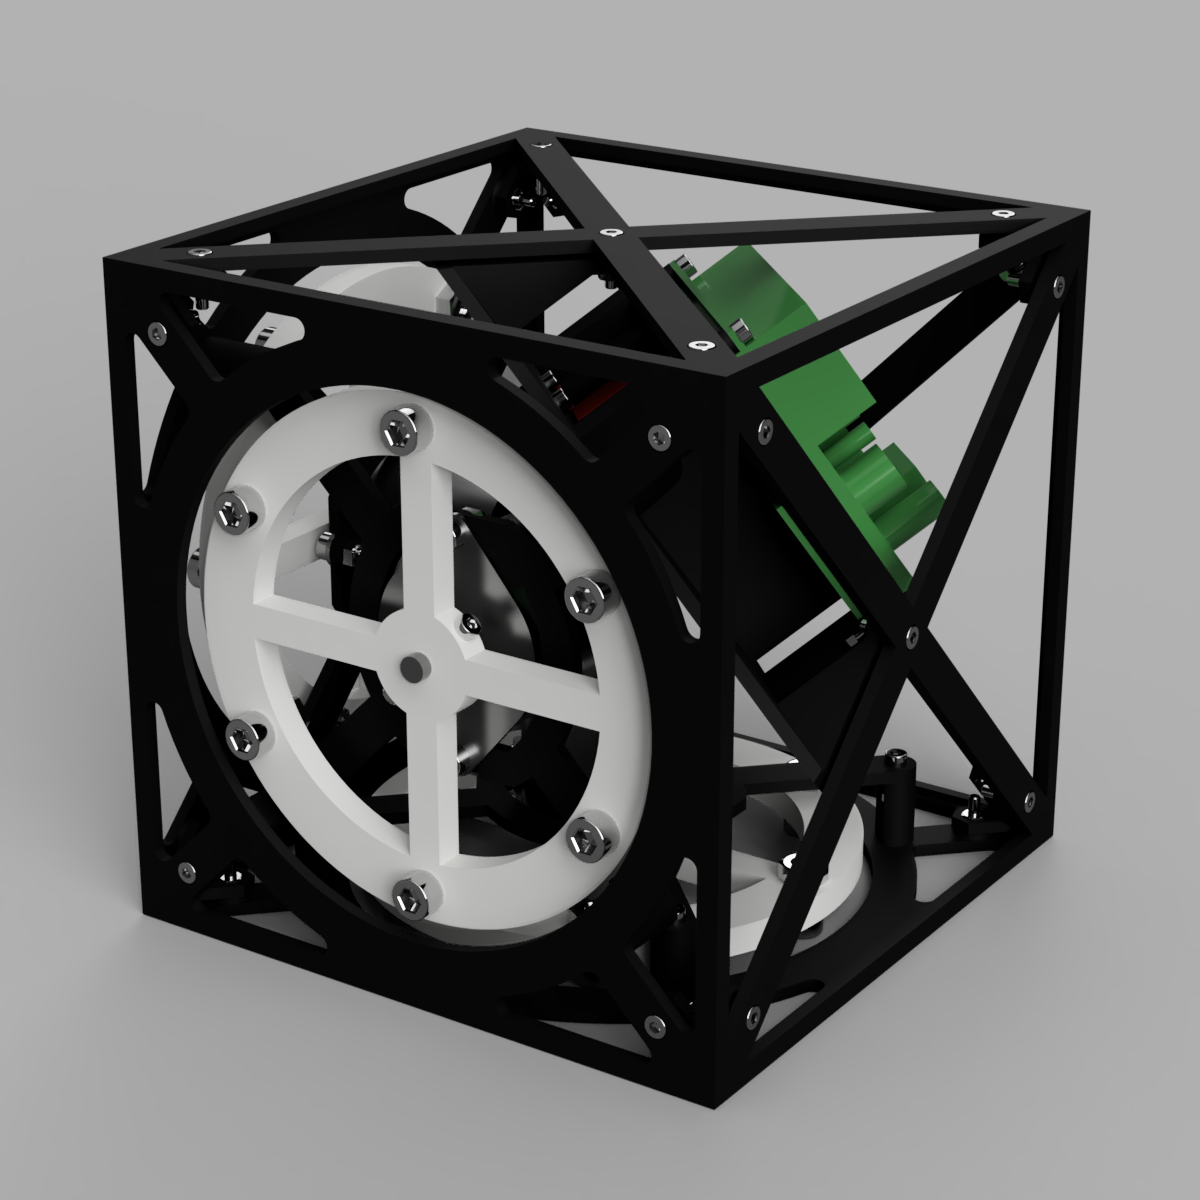
\includegraphics[width=0.6\textwidth]{cubilox_mk1_render.png}\par
  \vspace{1.2cm}
  {\large Technical Documentation\par}
  \vspace{0.4cm}
  {\large William Rosenberg\par}
  \vspace{0.4cm}
  {\large 2026\par}
  \vfill
  {\small This document is licensed under the Creative Commons Attribution 4.0
  International License (CC BY 4.0).\par}
\end{titlepage}

\pagenumbering{roman}
\chapter*{Abstract}
\addcontentsline{toc}{chapter}{Abstract}

The Cubilox Mk1 is a self-balancing cube that can stand on one of its edges or on one of its
corners (vertices). Three reaction wheels, each driven by a brushless Nidec~24H motor, are mounted
inside a 3D-printed frame. By accelerating and decelerating these wheels, the cube produces
reaction torques that keep its centre of mass above the edge or the corner it is standing on.
An ESP32 microcontroller estimates the orientation of the cube from an inertial measurement unit
(IMU) and runs two controllers: a single-axis controller for the edge and a three-dimensional
controller for the vertex, which separates the tilt motion from the rotation about the vertical
axis.

The project was designed and built entirely by the author: the mechanical parts were designed in
Fusion~360 and printed in PLA, the electronics were soldered on a prototype board, and the firmware
was written from scratch. It was inspired by the Cubli of ETH Zurich~\cite{gajamohan2012cubli,
gajamohan2013cubli} and, more directly, by the self-balancing cube of remrc~\cite{remrc_cube}.

This document describes the working principle, the mechanical and electrical design, the firmware
and its control laws, how to build, flash, calibrate and tune the cube, the results that were
achieved, and the lessons learned during development. The final version balances on its edge and,
after a calibration by hand, on its vertex for several minutes.

\tableofcontents
\listoffigures
\listoftables
\cleardoublepage
\pagenumbering{arabic}

\chapter{Introduction and Inspiration}
\label{ch:introduction}

\section{Motivation}

The Cubilox Mk1 is the author's first large electronics project. Before it, only small Arduino
projects had been built. The idea for the cube goes back several years, to a video of the
\emph{Cubli}, a cube developed at the Institute for Dynamic Systems and Control of ETH Zurich that
can jump up and balance on its corner~\cite{gajamohan2012cubli,gajamohan2013cubli}. The goal was
to build a similar cube completely independently, and to learn the required electronics, control
engineering and mechanical design along the way.

While researching what such a cube needs, the author came across the self-balancing cube of
remrc~\cite{remrc_cube}. This project had a strong influence on the Cubilox Mk1: it uses the
same type of motor (Nidec~24H) and a similar general layout. Nevertheless, every part of the
Cubilox Mk1 was created by the author: all mechanical parts were designed from scratch, the
circuit was designed and soldered independently, and the firmware was written without using code
from other cube projects.

Because it is a first project of this size, not every solution is best practice, and some
decisions would be made differently today. These points are discussed openly in
\cref{ch:limitations,ch:outlook}. The cube works, and the knowledge gained here is the basis for
future projects.

\section{Scientific background: the Cubli}

The Cubli is a \SI{15}{cm} cube with reaction wheels mounted on three of its faces. By applying
controlled torques to the wheels, it balances on an edge or a corner; by spinning the wheels up and
braking them abruptly, it can even jump up from a resting position~\cite{gajamohan2012cubli}. In
the second publication, the multi-body dynamics of the Cubli are derived, its parameters are
identified, and corner balancing with a linear state feedback controller is demonstrated
experimentally~\cite{gajamohan2013cubli}. The Cubli can therefore be seen as a three-dimensional
version of the classical inverted pendulum, actuated purely by internal reaction wheels.

\section{Goals and scope of the Cubilox Mk1}

The goals of the project were:
\begin{itemize}
  \item a cube that balances on an edge using one reaction wheel,
  \item a cube that balances on a vertex using all three reaction wheels,
  \item a design that can be printed on a standard consumer 3D printer and built from easily
        available parts,
  \item self-written firmware that can be tuned and calibrated wirelessly over Bluetooth.
\end{itemize}
Jumping up from a resting position, as the Cubli does, was not a goal of the Mk1 (see
\cref{ch:outlook}).

\Cref{fig:render,fig:vertex_photo} show the CAD model and the finished cube balancing on its
vertex.

\begin{figure}[htbp]
  \centering
  \begin{subfigure}[b]{0.48\textwidth}
    \centering
    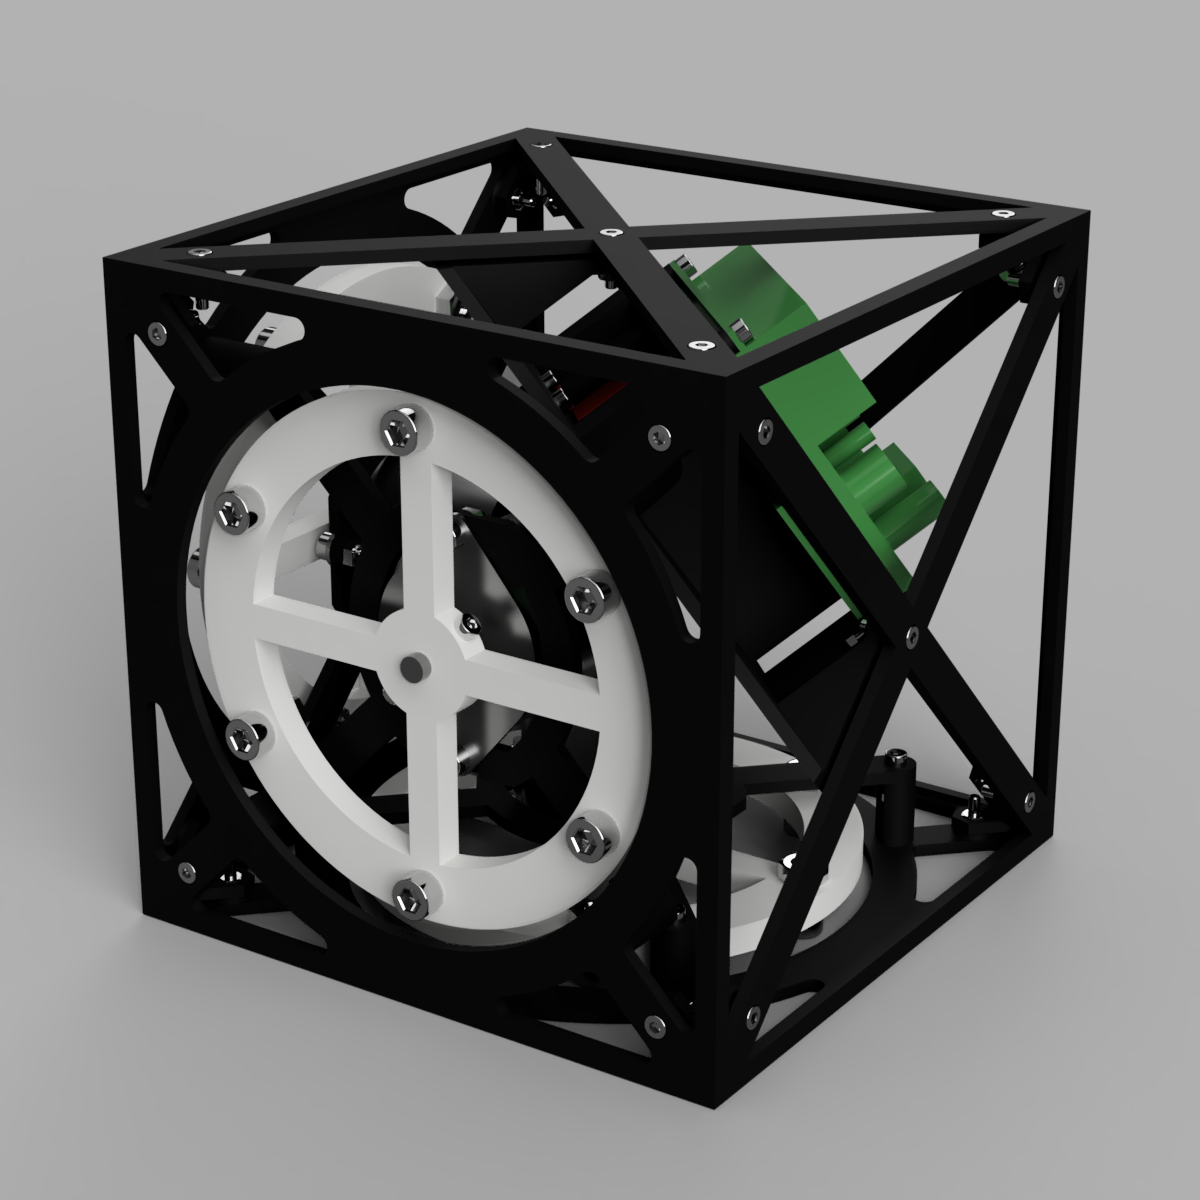
\includegraphics[width=\textwidth]{cubilox_mk1_render.png}
    \caption{Rendering of the CAD model.}
    \label{fig:render}
  \end{subfigure}\hfill
  \begin{subfigure}[b]{0.40\textwidth}
    \centering
    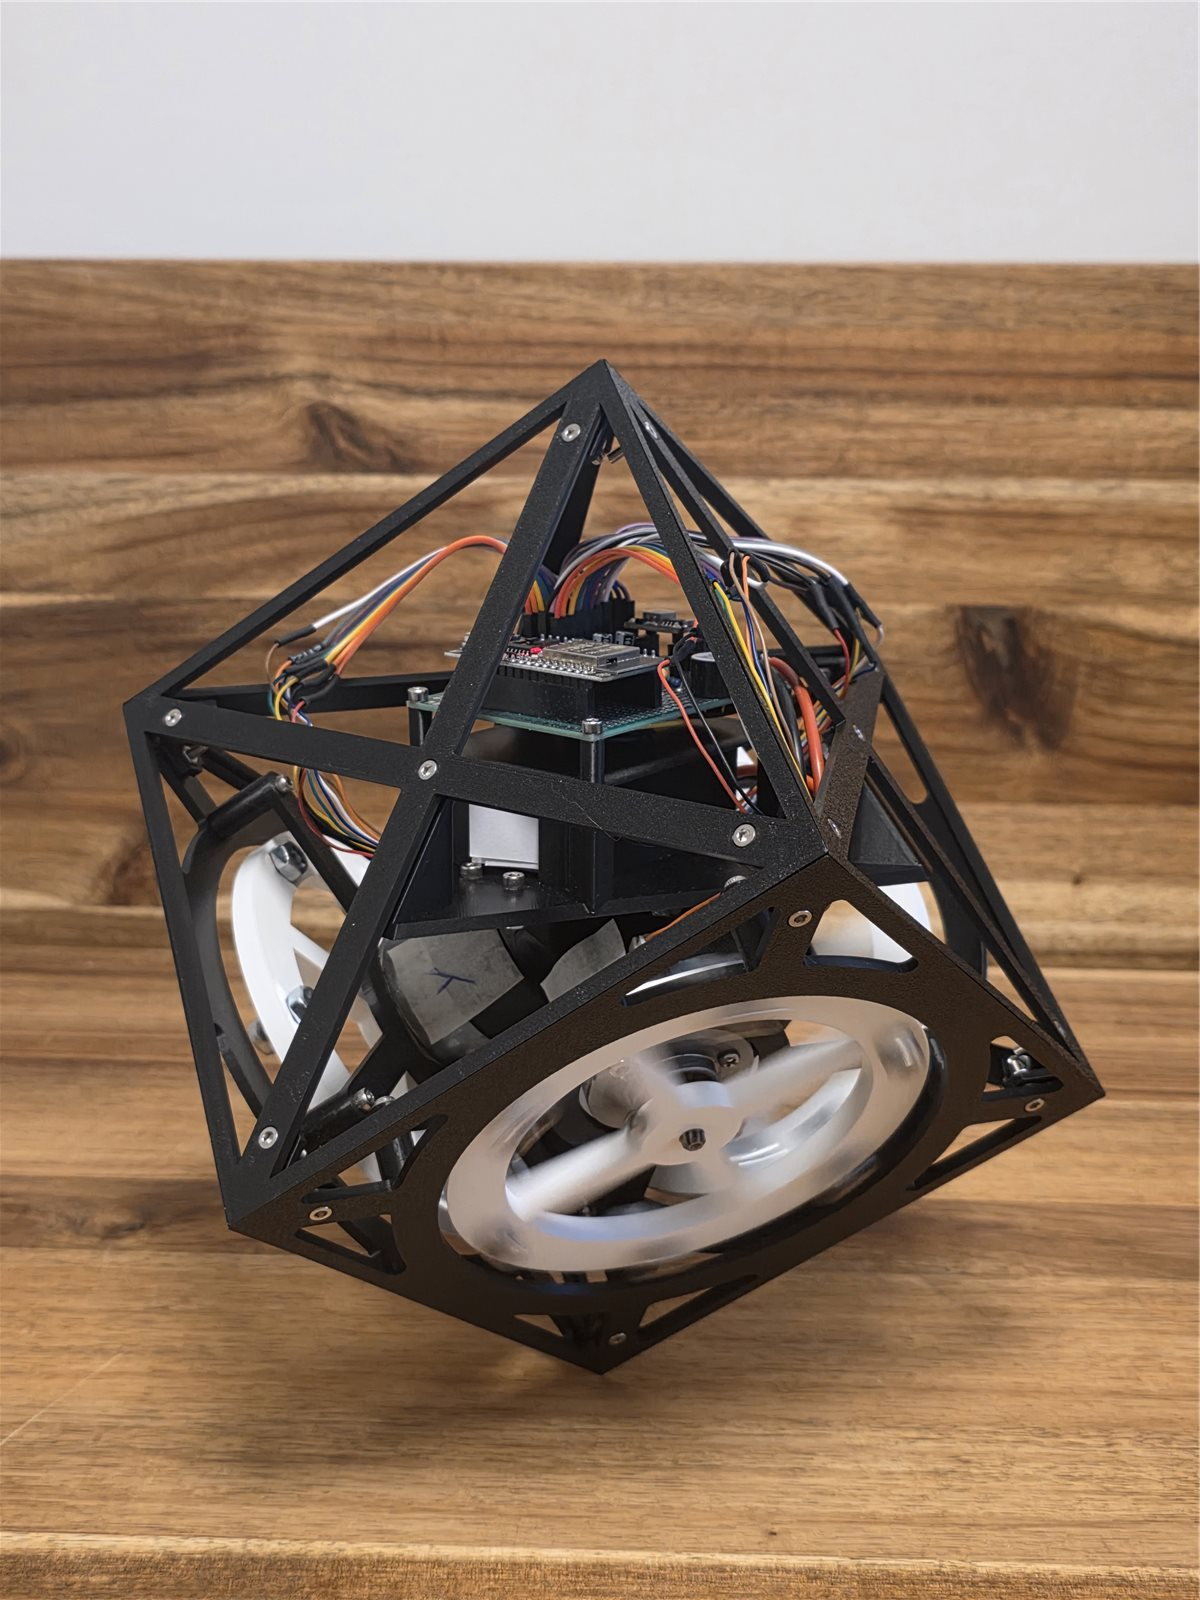
\includegraphics[width=\textwidth]{vertex_balance.jpg}
    \caption{The finished cube balancing on its vertex.}
    \label{fig:vertex_photo}
  \end{subfigure}
  \caption{The Cubilox Mk1: CAD model and built prototype.}
  \label{fig:overview}
\end{figure}

\section{Structure of this document}

\Cref{ch:principle} explains the physics of reaction wheel balancing.
\Cref{ch:mechanical,ch:electronics} describe the mechanical design and the electronics.
\Cref{ch:firmware} explains the firmware and the control laws in detail, followed by a getting
started guide (\cref{ch:getting_started}) and a tuning guide (\cref{ch:tuning}).
\Cref{ch:assembly} gives assembly instructions. \Cref{ch:results} presents the results and the
development history, \cref{ch:limitations} the limitations, and \cref{ch:outlook} the ideas for a
Mk2. The bill of materials and the third-party software are listed in the appendix.

\chapter{Working Principle and Physics}
\label{ch:principle}

This chapter explains why a cube can balance on an edge or a corner by means of internal reaction
wheels. The equations are simplified models that explain the behaviour and the structure of the
controllers in \cref{ch:firmware}; the gains of the Cubilox Mk1 were tuned experimentally and not
derived from an identified model.

\section{The cube as an inverted pendulum}

A cube resting on one of its edges or corners is an \emph{inverted pendulum}: its centre of mass
lies above the pivot, and any small deviation from the upright position produces a gravitational
torque that increases the deviation. For a cube with edge length $a$ and its centre of mass in the
geometric centre, the distance between pivot and centre of mass is
\begin{equation}
  l_\text{edge} = \frac{a}{\sqrt{2}} \qquad\text{and}\qquad l_\text{vertex} = \frac{\sqrt{3}}{2}\,a .
\end{equation}
For the Cubilox Mk1 with $a = \SI{157}{mm}$, and assuming the centre of mass in the geometric
centre, this gives $l_\text{edge} \approx \SI{111}{mm}$ and $l_\text{vertex} \approx \SI{136}{mm}$.
In the balanced edge position the faces adjacent to the edge are inclined by \ang{45}; in the
balanced vertex position the space diagonal through the pivot corner is vertical, so each face
normal makes an angle of $\arccos(1/\sqrt{3}) \approx \ang{54.7}$ with the vertical.

\section{Reaction wheels}

A reaction wheel is a flywheel driven by a motor that is fixed to the body. When the motor applies
a torque $\tau$ to the wheel, the wheel applies the opposite torque $-\tau$ to the body
(Newton's third law). Accelerating a wheel therefore rotates the cube in the opposite direction,
without any contact to the ground other than the pivot. The torque is only available while the
wheel speed changes: a wheel spinning at constant speed produces no torque. Since the speed of a
real motor is limited, a wheel cannot be accelerated in the same direction forever. This leads to
the need for wheel speed feedback, explained in \cref{sec:wheel_speed}.

The reaction torque is proportional to the moment of inertia of the wheel and its angular
acceleration. A large moment of inertia with little mass is achieved by placing mass far from the
axis; this is why the wheels of the Cubilox Mk1 carry screws and nuts on their rim
(\cref{sec:wheels}).

\section{Balancing on an edge (one axis)}
\label{sec:edge_model}

On an edge, the cube can only rotate about the edge, and one reaction wheel whose axis is parallel
to that edge is sufficient. Let $\theta$ be the tilt angle measured from the balance point,
$\Theta$ the moment of inertia of the cube about the edge, $m$ its mass, $g$ the gravitational
acceleration, $\Theta_w$ the moment of inertia of the wheel and $\omega_w$ the speed of the wheel
relative to the body. A simplified planar model is
\begin{align}
  \Theta\,\ddot\theta &= m g\, l_\text{edge} \sin\theta - \tau, \label{eq:edge_body}\\
  \Theta_w \left(\dot\omega_w + \ddot\theta\right) &= \tau, \label{eq:edge_wheel}
\end{align}
where $\tau$ is the motor torque acting on the wheel. Linearised around $\theta = 0$
($\sin\theta \approx \theta$), the uncontrolled system has a real positive eigenvalue
$\lambda = \sqrt{m g\, l_\text{edge}/\Theta}$: without control, a small deviation grows
exponentially and the cube falls.

A linear state feedback of the tilt angle, the tilt rate and the wheel speed stabilises the
system:
\begin{equation}
  u = K_1\,\theta + K_2\,\dot\theta + K_3\,\omega_w ,
  \label{eq:edge_law}
\end{equation}
where $u$ is the motor command. In the firmware, these three terms are the gains
\cmd{ek1}, \cmd{ek2} and \cmd{ek3} (\cref{sec:edge_controller}):
\begin{itemize}
  \item the \textbf{angle term} $K_1\theta$ pushes the cube back towards the balance point,
  \item the \textbf{rate term} $K_2\dot\theta$ damps the motion and prevents overshooting,
  \item the \textbf{wheel speed term} $K_3\omega_w$ keeps the wheel speed bounded.
\end{itemize}

\section{Why wheel speed feedback is needed}
\label{sec:wheel_speed}

If the balance point assumed by the controller differs slightly from the real one (for example
because the centre of mass is not exactly where it was expected), the cube needs a permanent
torque to stay upright. A permanent torque means a permanently accelerating wheel, which sooner or
later reaches its maximum speed; from then on, no torque is available and the cube falls. This is
called \emph{saturation}.

The wheel speed term solves this: when the wheel spins in one direction, the controller lets the
cube lean slightly to the other side, so that gravity provides the torque instead of the wheel,
and the wheel slows down again. In steady state $\dot\theta = 0$ and the motor command averages to
zero, so \cref{eq:edge_law} gives
\begin{equation}
  K_1\,\theta + K_3\,\omega_w \approx 0 .
  \label{eq:equilibrium}
\end{equation}
This relation is also the basis of the automatic trim (\cref{sec:trim}): if the wheel keeps turning
in one direction, the setpoint of the angle is shifted until the wheel rests on average.

\section{Balancing on a vertex (three axes)}
\label{sec:vertex_model}

On a vertex, the cube can tilt in any direction, and three reaction wheels with mutually
orthogonal axes are used. The orientation error is now a vector. Let $\vect{r}$ be the unit vector
of the gravity direction in the balanced position and $\vect{n}$ the current gravity direction,
both expressed in the body frame of the cube (\cref{fig:vertex_vectors}). For small angles, the
cross product
\begin{equation}
  \vect{e} = \vect{n} \times \vect{r}
  \label{eq:vertex_error}
\end{equation}
is the rotation vector (axis times angle, in radians) that describes the tilt of the cube. Its
magnitude is the tilt angle and its direction is the axis about which the cube must be rotated
back.

Rotations about $\vect{r}$, the vertical axis (\emph{yaw}), are special: gravity produces no torque
about this axis, so a yaw rotation does not affect the balance at all. The vertex controller
therefore splits every vector quantity $\vect{v}$ into a tilt part and a yaw part:
\begin{equation}
  \vect{v}_\text{yaw} = (\vect{v}\cdot\vect{r})\,\vect{r}, \qquad
  \vect{v}_\text{tilt} = \vect{v} - \vect{v}_\text{yaw}.
  \label{eq:split}
\end{equation}

\begin{figure}[htbp]
  \centering
  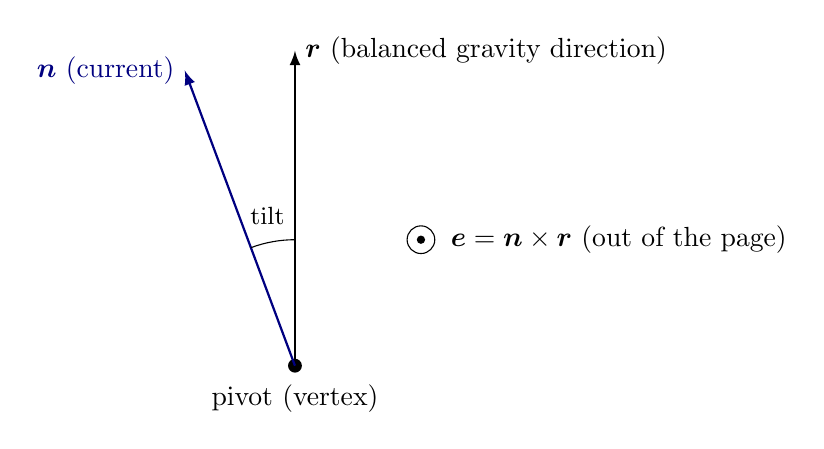
\begin{tikzpicture}[>=latex, thick]
    \fill (0,0) circle (2.5pt) node[below=3pt] {pivot (vertex)};
    \draw[->] (0,0) -- (0,4) node[right] {$\vect{r}$ (balanced gravity direction)};
    \draw[->, NavyBlue] (0,0) -- (-1.4,3.75) node[left] {$\vect{n}$ (current)};
    \draw[thin] (0,1.6) arc (90:110.5:1.6);
    \node at (-0.35,1.9) {\small tilt};
    \draw[thin] (1.6,1.6) circle (5pt);
    \fill (1.6,1.6) circle (1.5pt);
    \node[right] at (1.85,1.6) {$\vect{e} = \vect{n}\times\vect{r}$ (out of the page)};
  \end{tikzpicture}
  \caption{Tilt error at the vertex: $\vect{r}$ is the gravity direction in the calibrated
    balance position, $\vect{n}$ the current one, both measured in the body frame. Their cross
    product is the rotation vector of the tilt.}
  \label{fig:vertex_vectors}
\end{figure}

\section{Angular momentum about the vertical axis}
\label{sec:yaw_physics}

The wheels store angular momentum $\vect{h}$. Its tilt part is controlled exactly like the wheel
speed on the edge: gravity can remove it if the cube leans slightly. Its yaw part, however, cannot
be removed by gravity. If the controller fed back the yaw momentum in the same way as the tilt
momentum, it would form a positive feedback loop: more yaw momentum would cause a larger command
along the yaw axis, which would accelerate the wheels further. This effect was observed on the
real cube (\cref{sec:history}): with a negative yaw gain the yaw momentum grew exponentially with a
time constant of about \SI{2.4}{s} until the motors saturated, and the cube was visibly rotating
about its vertical axis.

The vertex controller therefore uses separate gains for the yaw part: a damping term on the yaw
rate and a term that slowly reduces the yaw momentum of the wheels. The reaction is transferred
to the ground through the friction at the pivot.

\section{Sensing the orientation}

The orientation is measured with an IMU that contains a three-axis accelerometer and a three-axis
gyroscope:
\begin{itemize}
  \item The \textbf{accelerometer} measures the gravity direction, which directly gives the tilt.
        However, it also measures every linear acceleration of the sensor. Each time the wheels
        accelerate, the cube jerks slightly, and the measured direction is disturbed.
  \item The \textbf{gyroscope} measures the angular rate. It is fast and not disturbed by linear
        accelerations, but integrating it to get an angle accumulates a slowly growing error
        (drift).
\end{itemize}
A \emph{complementary filter} combines both: the gyroscope is integrated for fast changes, and the
accelerometer slowly corrects the drift. With a filter constant $\alpha$ close to 1,
\begin{equation}
  \hat\theta_k = \alpha\left(\hat\theta_{k-1} + \omega\,\Delta t\right) + (1-\alpha)\,\theta_\text{acc} .
  \label{eq:cf}
\end{equation}
The firmware uses this filter on the edge and a three-dimensional version of it on the vertex
(\cref{sec:sensor_processing}).

\chapter{Mechanical Design}
\label{ch:mechanical}

\section{Overview}

All mechanical parts of the Cubilox Mk1 were designed by the author in Fusion~360 and printed in
standard PLA on a Bambu Lab A1 printer, using the default settings of the Bambu Studio slicer.
The frame of the cube consists of three motor walls carrying the motors and reaction wheels, three
side walls, and eight corner mounts that join the walls with M3 screws and nuts. The electronics
sit on a base plate inside the cube. \Cref{tab:printed_parts} lists all printed parts and
\cref{tab:mech_params} the key parameters.

\begin{table}[htbp]
  \centering
  \caption{3D-printed parts of the Cubilox Mk1.}
  \label{tab:printed_parts}
  \begin{tabular}{lcl}
    \toprule
    Part & Quantity & Function \\
    \midrule
    \cmd{motor\_wall}            & 3 & frame face carrying one motor and its reaction wheel \\
    \cmd{side\_wall}             & 3 & frame face without motor \\
    \cmd{corner\_mount}          & 8 & joins the walls at the corners (M3 nuts press-fit) \\
    \cmd{motor\_mount}           & 6 & holds a motor (fixed with M4 screws) \\
    \cmd{flywheel}               & 3 & reaction wheel \\
    \cmd{sensor\_mount}          & 1 & holds the IMU near the centre of the cube \\
    \cmd{electronic\_base\_plate} & 1 & carries the electronics \\
    \cmd{intermediate\_plate}    & 1 & encloses the battery and carries the circuit board \\
    \bottomrule
  \end{tabular}
\end{table}

\begin{table}[htbp]
  \centering
  \caption{Key mechanical parameters.}
  \label{tab:mech_params}
  \begin{tabular}{ll}
    \toprule
    Parameter & Value \\
    \midrule
    Total mass of the cube                         & \SI{1036}{g} \\
    Mass of one reaction wheel incl.\ screws and nuts & \SI{76.4}{g} \\
    Mass of the battery                            & approx.\ \SI{80}{g} \\
    PLA used for all printed parts                 & \SI{283}{g} \\
    Total print time                               & approx.\ \SI{14}{h} \\
    Edge length of the cube                        & \SI{157}{mm} \\
    \bottomrule
  \end{tabular}
\end{table}

\section{Design for 3D printing}

All parts were designed to be printable without or with very few supports. Overhangs are kept at
printable angles, and horizontal holes and nut pockets use teardrop or pointed shapes, so that the
upper side of the opening is built as a self-supporting overhang instead of a flat bridge.
\Cref{fig:print_optimization} shows two examples.

\begin{figure}[htbp]
  \centering
  \begin{subfigure}[b]{0.42\textwidth}
    \centering
    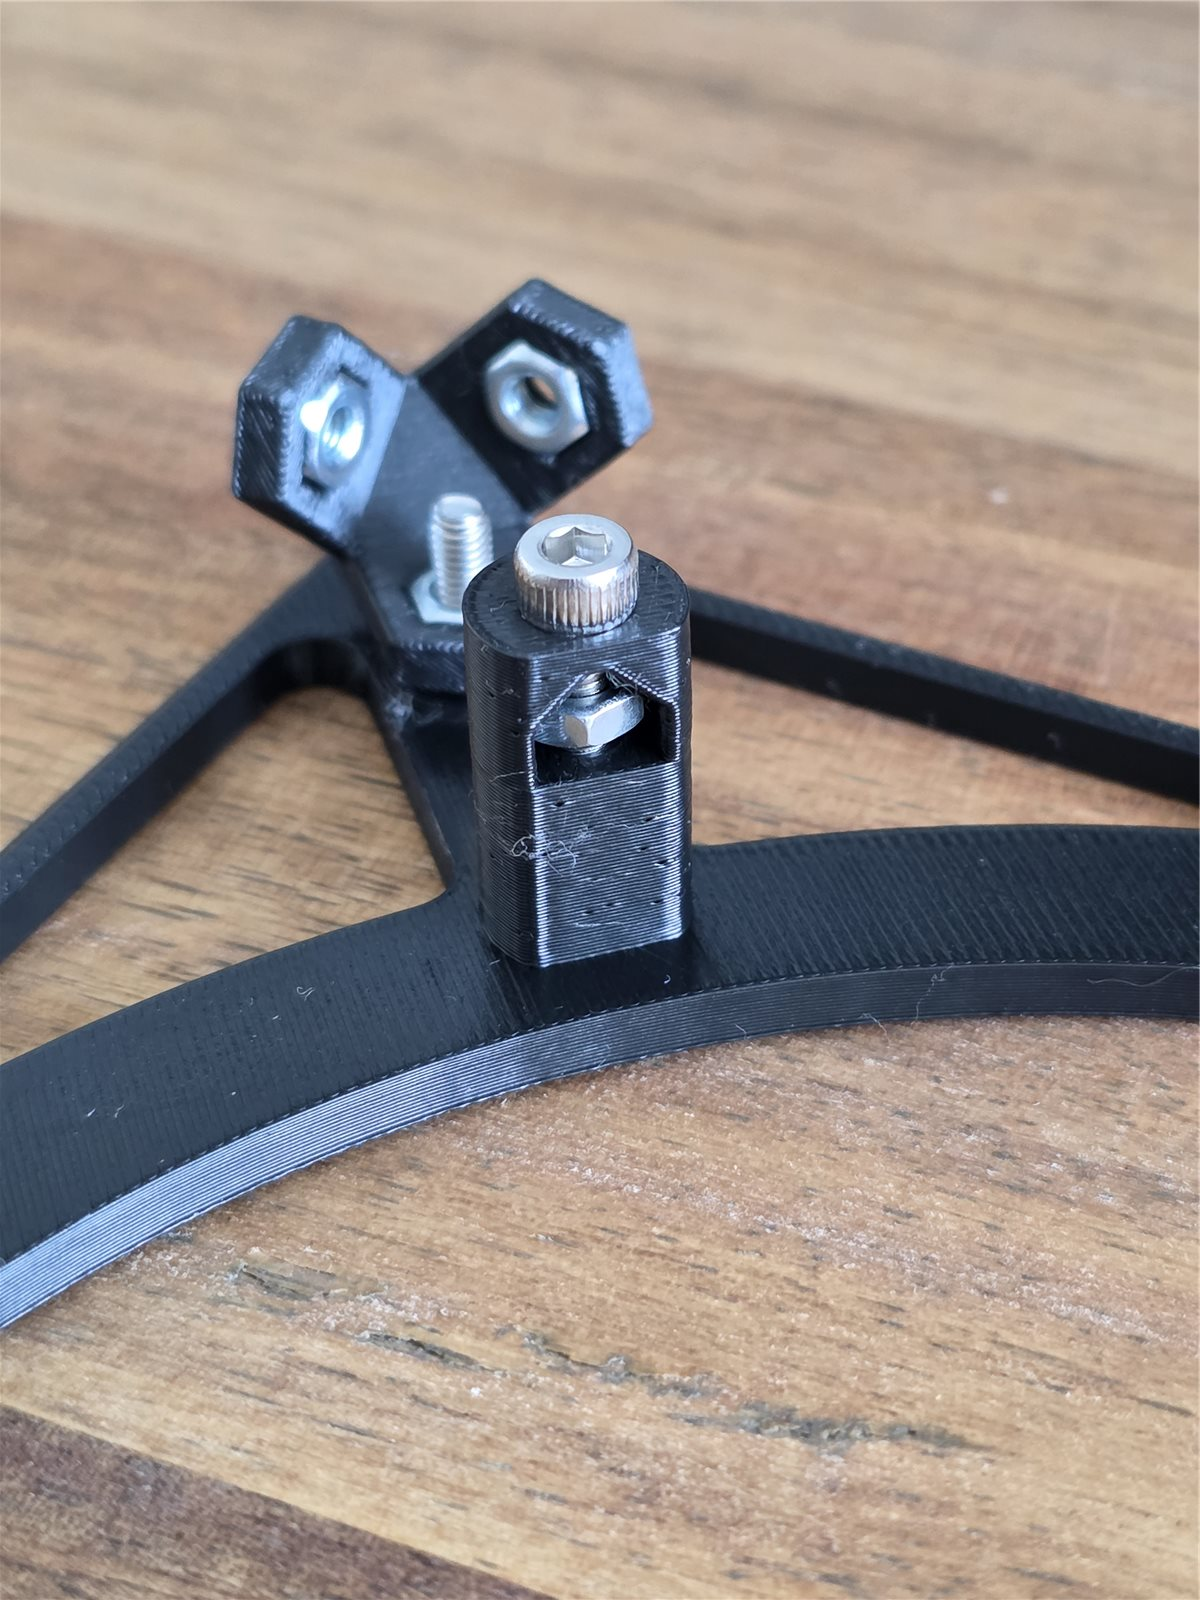
\includegraphics[width=\textwidth]{print_optimization_example_1.jpg}
    \caption{Nut pocket with a pointed roof, printable without supports.}
    \label{fig:print_opt_1}
  \end{subfigure}\hfill
  \begin{subfigure}[b]{0.42\textwidth}
    \centering
    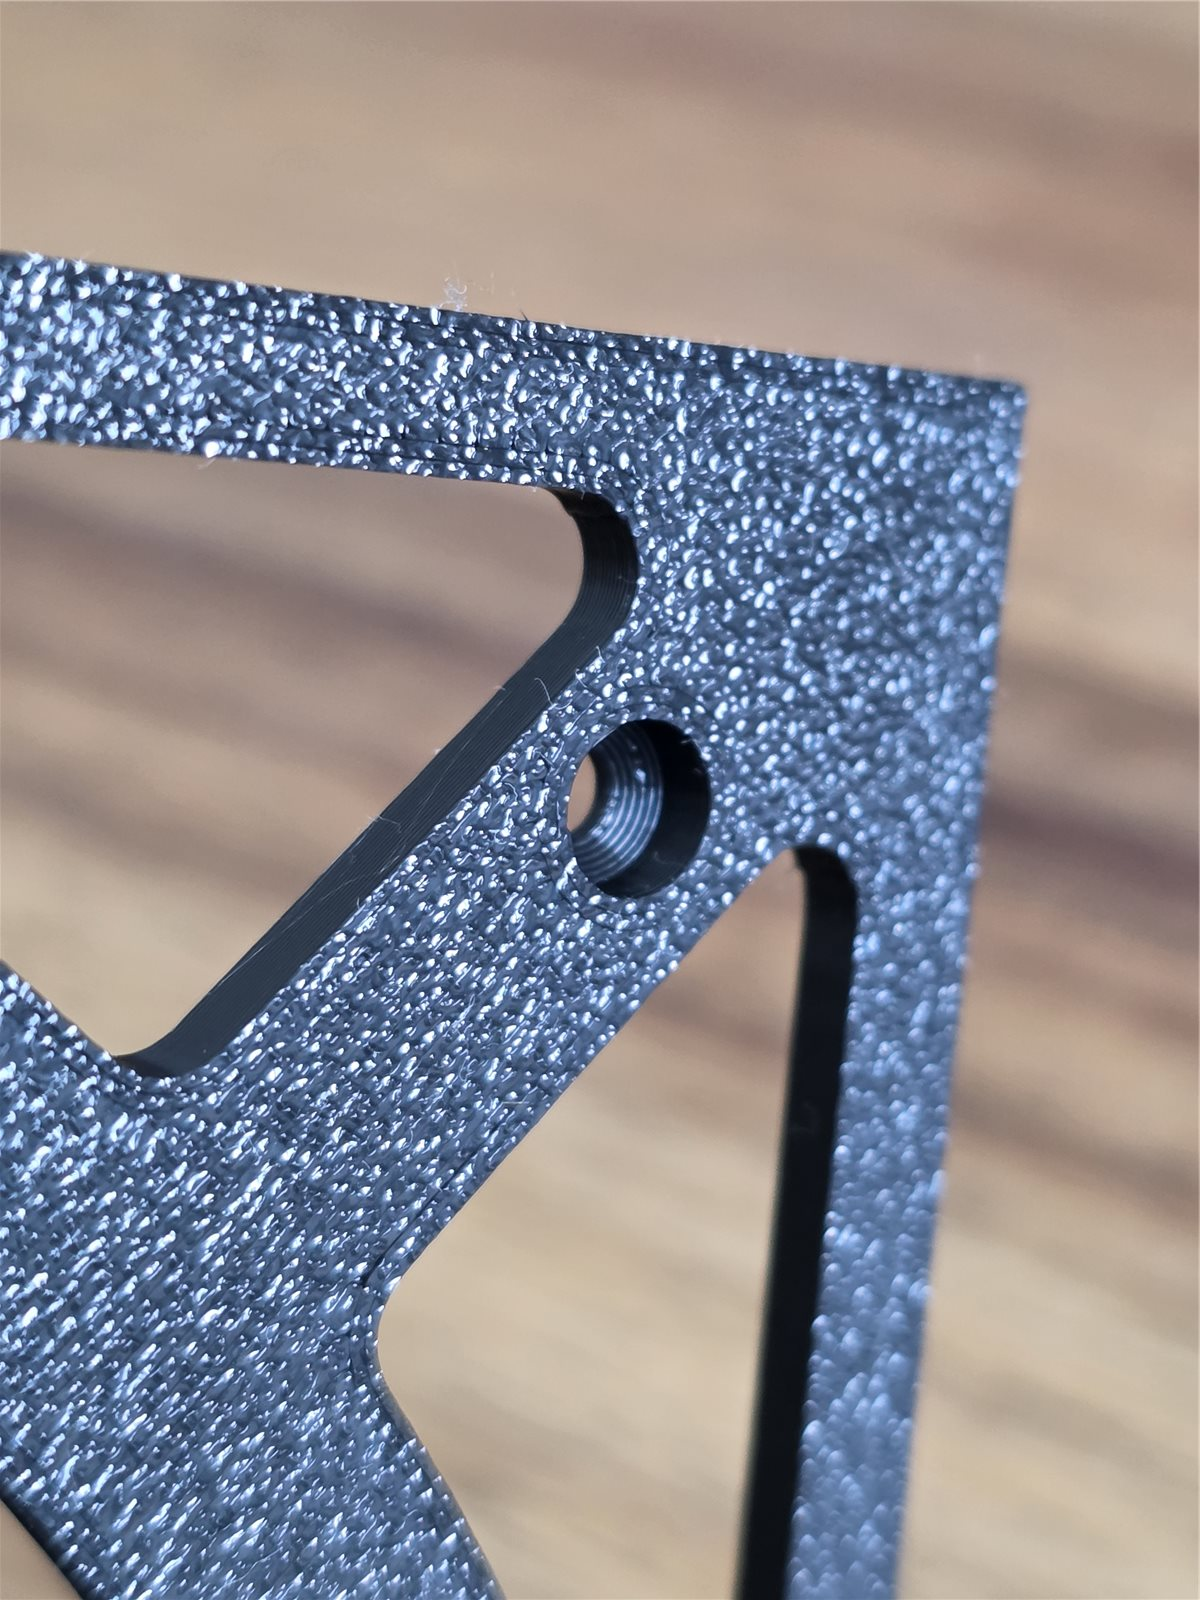
\includegraphics[width=\textwidth]{print_optimization_example_2.jpg}
    \caption{Detail of a printed frame part with a screw hole and cut-out.}
    \label{fig:print_opt_2}
  \end{subfigure}
  \caption{Examples of geometry optimised for FDM printing.}
  \label{fig:print_optimization}
\end{figure}

\section{Reaction wheels}
\label{sec:wheels}

Each reaction wheel (\cref{fig:wheel}) is a printed ring with four spokes. Six M6 screws, each with
two M6 nuts, are mounted on the rim. They add mass at the largest possible radius and thereby
increase the moment of inertia of the wheel without making the wheel much heavier. One complete
wheel including all screws and nuts weighs \SI{76.4}{g}. The hub is clamped onto the motor shaft
with two screws.

\begin{figure}[htbp]
  \centering
  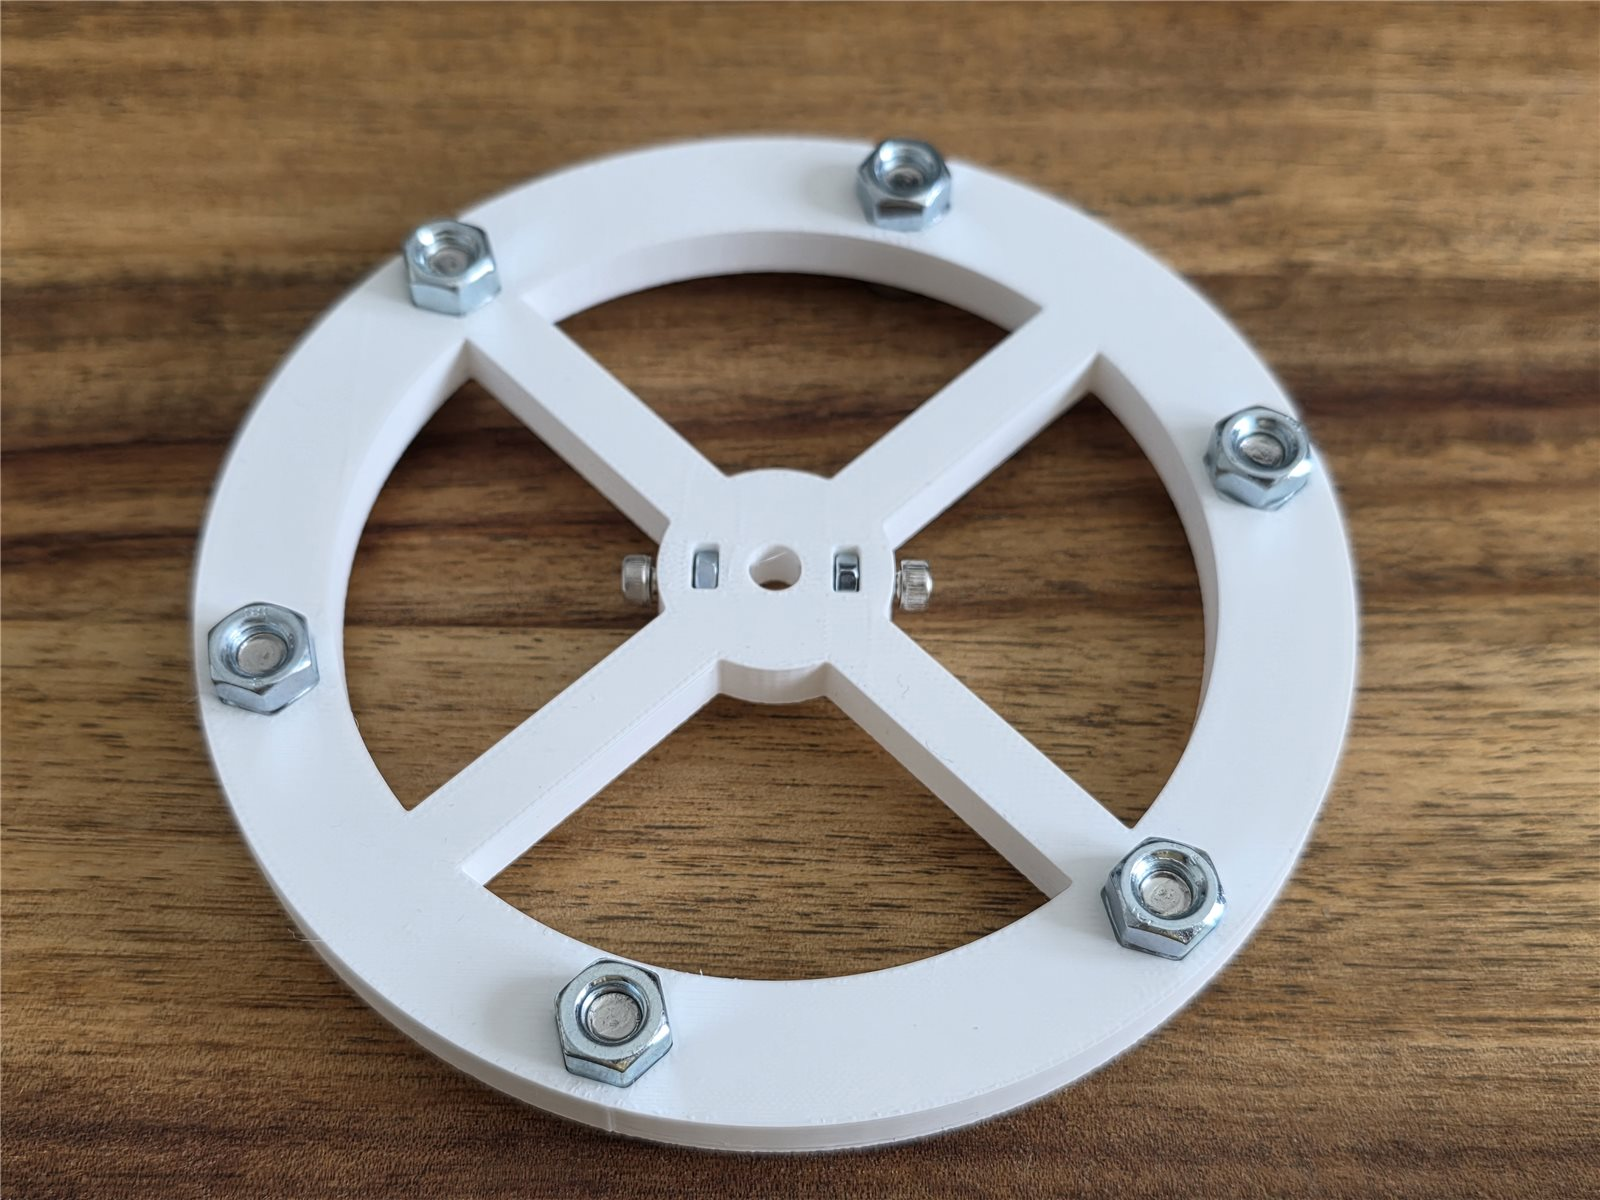
\includegraphics[width=0.6\textwidth]{reaction_wheel_with_bolts.jpg}
  \caption{Reaction wheel with the M6 screws and nuts on its rim and the two clamping screws at the
    hub.}
  \label{fig:wheel}
\end{figure}

The wheel must sit exactly perpendicular on the motor shaft. A wheel that wobbles causes
vibrations, which disturb the IMU, and it can rub against the frame. During development, a wheel
that rubbed against the frame because of a loose screw produced cracking noises and shocks that
shortened the balancing time considerably (\cref{sec:history}).

\section{Sensor mount and sensor position}

The IMU is mounted as close as possible to the geometric centre of the cube, with each of its
three axes aligned with the axis of one motor. This is why the motors are called X, Y and Z: motor X
rotates the cube about the sensor's X axis, and so on. Placing the sensor near the centre keeps the
accelerations it measures during rotations small.

The sensor mount (\cref{fig:sensor_mount}) was created with the generative design function of
Fusion~360. Despite its organic shape, it can be printed with remarkably little support material.

\begin{figure}[htbp]
  \centering
  \begin{subfigure}[b]{0.36\textwidth}
    \centering
    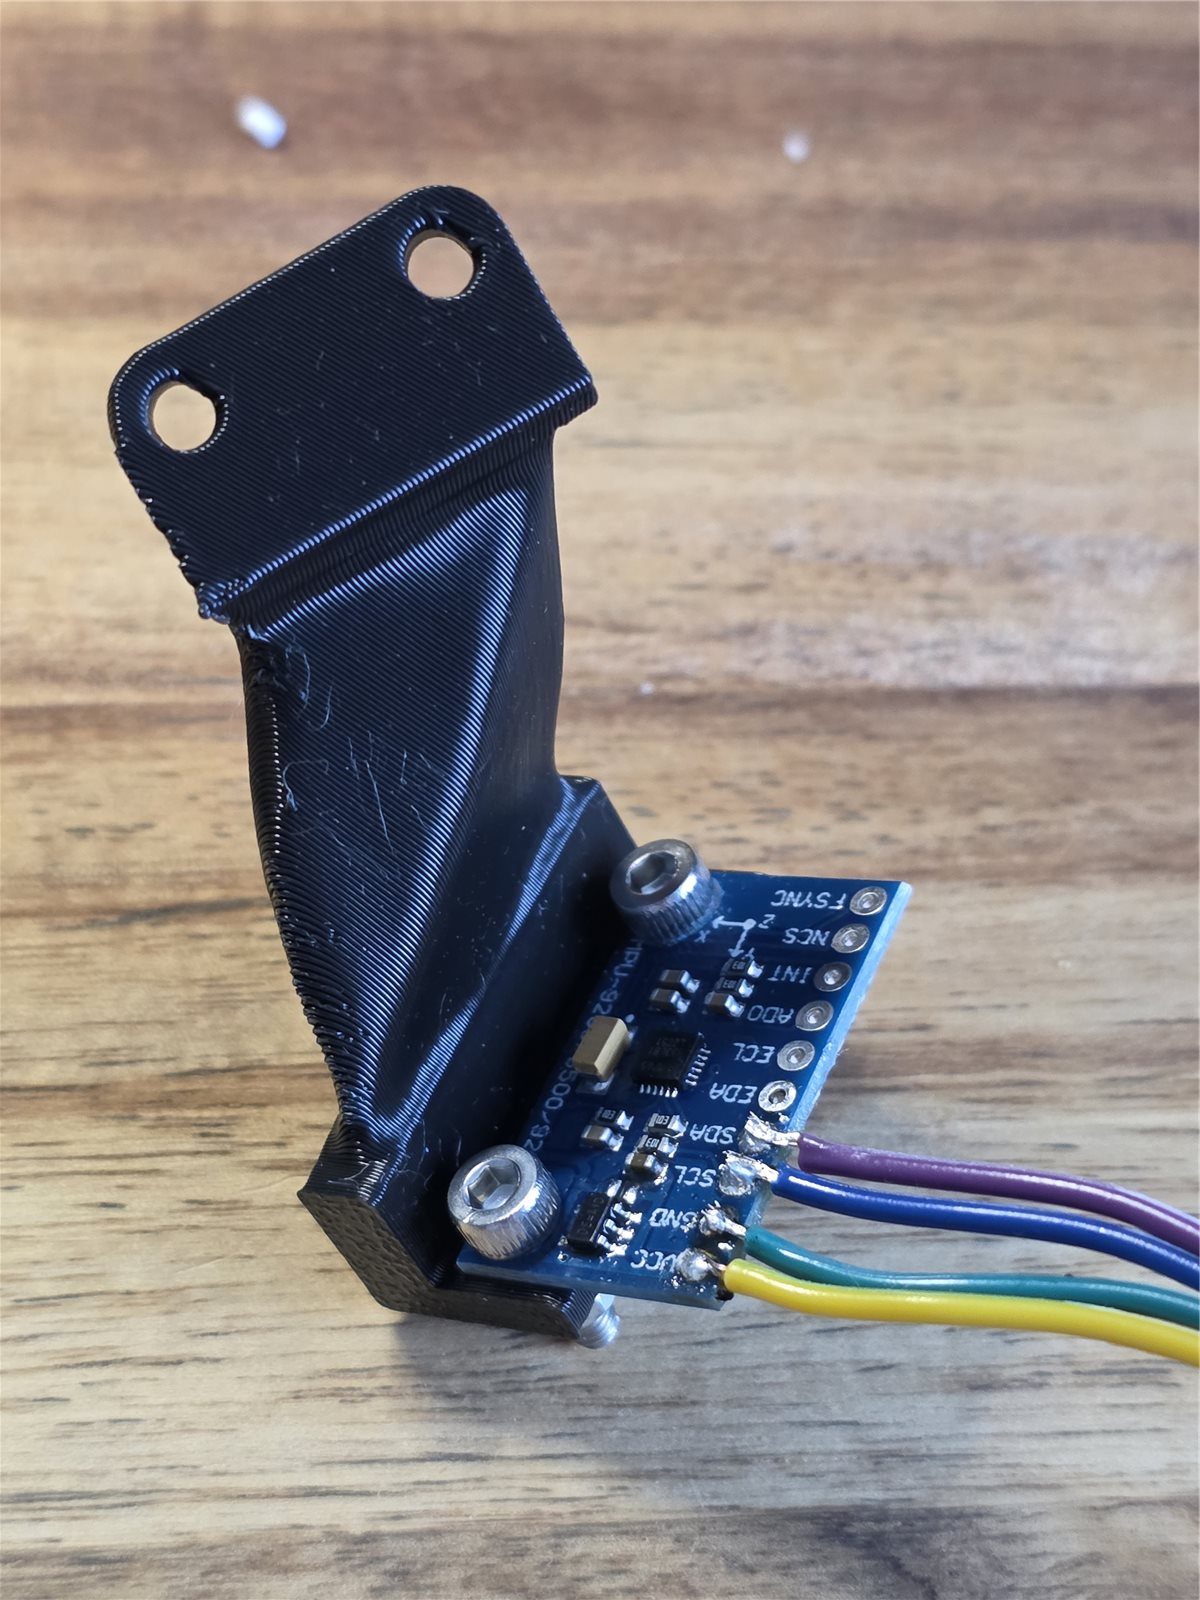
\includegraphics[width=\textwidth]{mpu_with_holder.jpg}
    \caption{Printed sensor mount with the IMU board.}
    \label{fig:mpu_holder}
  \end{subfigure}\hfill
  \begin{subfigure}[b]{0.56\textwidth}
    \centering
    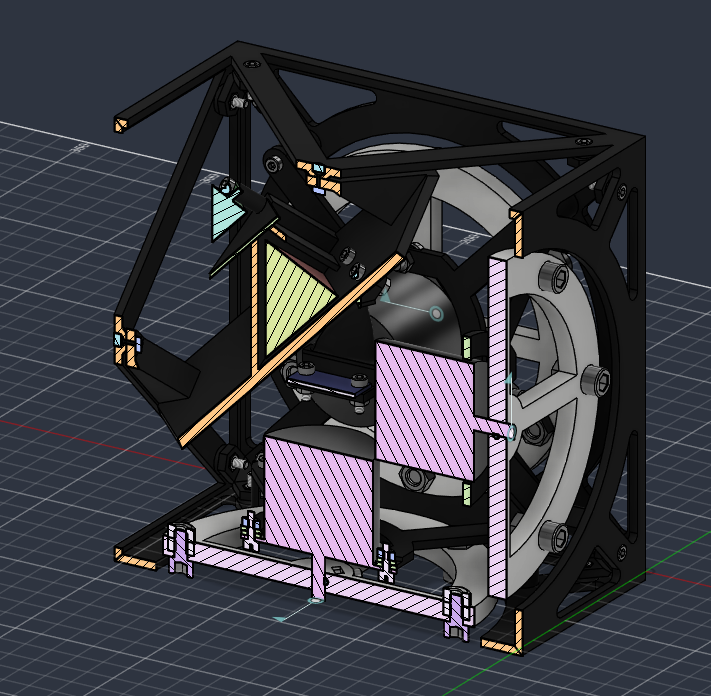
\includegraphics[width=\textwidth]{sensor_position_cad.png}
    \caption{Section view of the CAD model showing the sensor position.}
    \label{fig:sensor_cad}
  \end{subfigure}
  \caption{Sensor mount and position of the IMU inside the cube.}
  \label{fig:sensor_mount}
\end{figure}

\section{Battery compartment}

The battery sits in a compartment that is closed by the intermediate plate. The circuit board is
screwed on top of this plate with some clearance, so that the cables underneath the board are not
crushed. The compartment is padded with cardboard and folded paper. The padding
fixes the battery in place and absorbs some of the shock when the cube falls over. The
accelerations during a normal fall are usually not high enough to damage the battery, but
securing a LiPo battery against shocks is good practice.

\chapter{Electronics}
\label{ch:electronics}

\section{Overview}

All electronic components are soldered onto a \qtyproduct{60 x 80}{mm} prototype board
(\cref{fig:pcb}). The main components are:
\begin{itemize}
  \item an \textbf{ESP32 development board} (HW-394, ESP32-32D module, USB-C) as the
        microcontroller,
  \item an \textbf{IMU breakout board} labelled \enquote{MPU-9250/6500/9255} (MPU-6500 family,
        three-axis accelerometer and gyroscope), connected via I\textsuperscript{2}C and read with
        the MPU6050\_light library~\cite{mpu6050light}, whose register accesses are compatible
        with this sensor,
  \item three \textbf{Nidec~24H brushless motors} with integrated driver and encoder; the
        \textbf{8-pin version} is required (the author first bought the 12-pin version, which does
        not fit this design),
  \item a \textbf{3S LiPo battery} (\SI{11.1}{V} nominal, \SI{12.6}{V} fully charged,
        \SI{1000}{mAh}) with an XT30 connector,
  \item a \textbf{mini DC-DC buck converter} (input \SIrange{5}{30}{V}, output \SI{5}{V}),
  \item an \textbf{active \SI{5}{V} buzzer} switched by a 2N2222 transistor,
  \item a \textbf{voltage divider} for measuring the battery voltage, and buffer capacitors.
\end{itemize}
The board carries three 8-pin headers for the motor cables and a 4-pin header for the IMU.
The complete schematic is shown in \cref{fig:schematic}; all connections are also listed in the
file \nolinkurl{hardware/electronics/wiring.md} of the repository.

The schematic was the author's first project in KiCad and is therefore not as clearly arranged as
it could be. Two details differ from the built cube: the transistor symbol is labelled 2N2219,
while a 2N2222 is used, and the motors are numbered 1--3 instead of X, Y, Z
(Nidec24H1~=~motor~X, Nidec24H2~=~motor~Z, Nidec24H3~=~motor~Y).

\begin{landscape}
\begin{figure}[p]
  \centering
  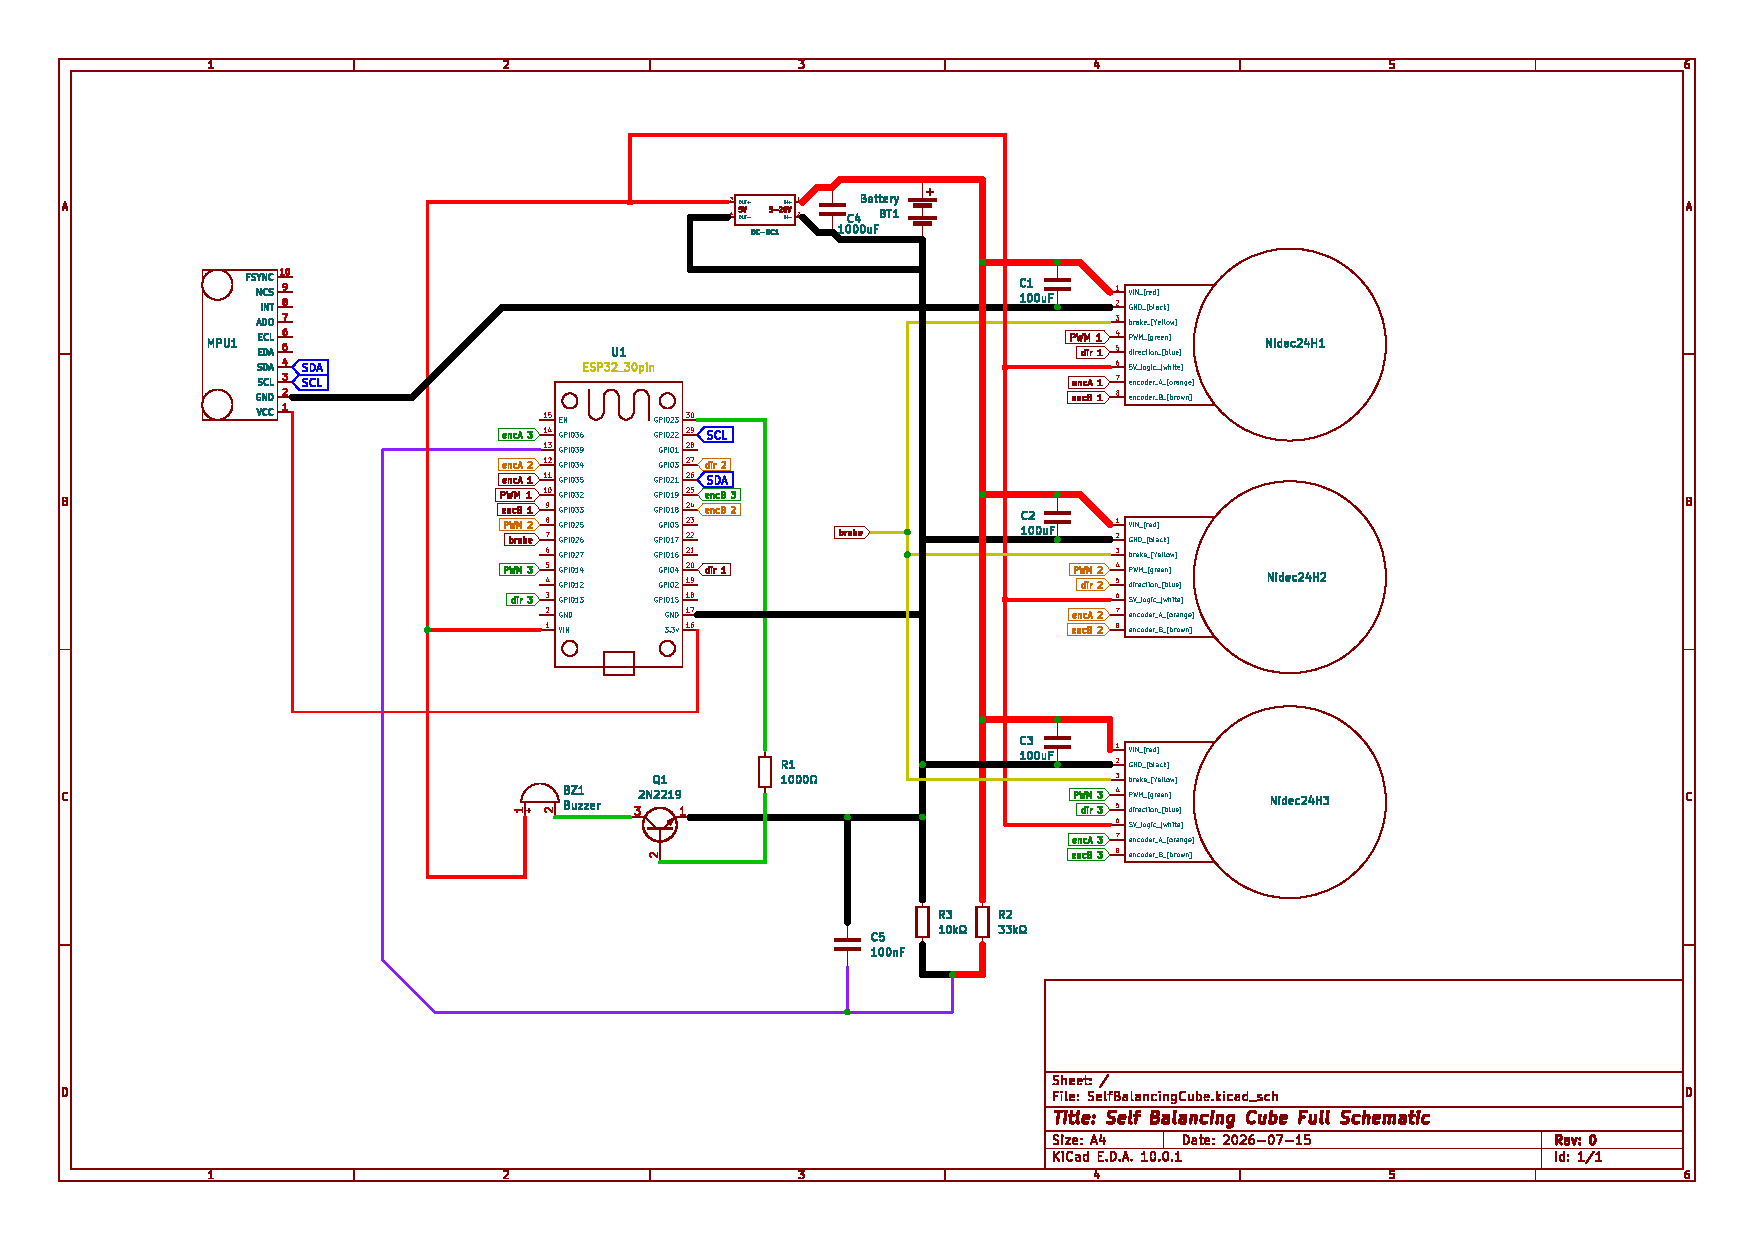
\includegraphics[width=\linewidth,height=0.88\textheight,keepaspectratio]{cubilox_mk1_schematic.pdf}
  \caption{Complete schematic of the Cubilox Mk1 (KiCad). The transistor Q1 is a 2N2222 in the
    built cube.}
  \label{fig:schematic}
\end{figure}
\end{landscape}

\section{Power supply}

The battery feeds a common \SI{12}{V} rail, which supplies the three motors directly (red wire,
VIN) and the buck converter. The buck converter produces \SI{5}{V} for the VIN pin of the ESP32
board and for the logic supply of the motors (white wire). The ESP32 board generates the
\SI{3.3}{V} for the IMU with its on-board regulator. All grounds are connected to one common GND
rail.

\begin{table}[htbp]
  \centering
  \caption{Power distribution.}
  \label{tab:power}
  \begin{tabularx}{\textwidth}{lX}
    \toprule
    Rail & Consumers \\
    \midrule
    Battery (\SIrange{11.1}{12.6}{V}) & motor power (VIN) of all three motors, buck converter input,
                                        voltage divider \\
    \SI{5}{V} (buck converter)        & ESP32 VIN, motor logic supply, buzzer \\
    \SI{3.3}{V} (ESP32 board)         & IMU \\
    \bottomrule
  \end{tabularx}
\end{table}

\subsection{Buffer capacitors}

The motors draw short, high current peaks whenever they accelerate or reverse, which happens
continuously while balancing. Because of the resistance and inductance of the battery and the
wires, these peaks cause short voltage dips on the supply rails. Such dips can disturb or reset
the ESP32 and the motor drivers. Three types of capacitors reduce this effect:
\begin{itemize}
  \item \textbf{C4, \SI{1000}{\micro F} electrolytic}, directly at the battery input: a large
        reservoir that supplies the current peaks of all motors together and smooths the main
        rail.
  \item \textbf{C1--C3, \SI{100}{\micro F} electrolytic}, one at the supply of each motor: local
        reservoirs close to the consumers, so that the peak current of one motor does not have to
        flow through the whole wiring and disturb the others.
  \item \textbf{C5, \SI{100}{nF} ceramic}, at the measuring point of the voltage divider: a small
        capacitor that filters noise on the ADC input (see \cref{sec:divider}).
\end{itemize}

\section{Battery voltage measurement}
\label{sec:divider}

The ESP32's analogue-to-digital converter (ADC) can only measure voltages up to about
\SI{3.3}{V}, while the battery reaches \SI{12.6}{V}. A voltage divider scales the battery voltage
down:
\begin{equation}
  V_\text{pin} = V_\text{bat}\,\frac{R_3}{R_2 + R_3}
             = V_\text{bat}\,\frac{\SI{10}{k\ohm}}{\SI{33}{k\ohm} + \SI{10}{k\ohm}}
             \approx 0.233\,V_\text{bat}.
\end{equation}
For a full battery, $V_\text{pin} = \SI{12.6}{V} \times 0.233 \approx \SI{2.93}{V}$, safely below
the limit. The firmware reverses this calculation by multiplying the measured pin voltage by
$(R_2+R_3)/R_3 = 4.3$ (\cref{lst:battery}). The upper resistor of \SI{33}{k\ohm} is built from
three resistors in series (\SI{20}{k\ohm} + \SI{10}{k\ohm} + \SI{3.3}{k\ohm}), because no single
\SI{33}{k\ohm} resistor was at hand.

The high resistance values keep the current through the divider small,
$I = \SI{12.6}{V} / \SI{43}{k\ohm} \approx \SI{0.29}{mA}$, so the divider hardly drains the battery.
Together with the source resistance of the divider,
$R_2 \parallel R_3 \approx \SI{7.7}{k\ohm}$, the \SI{100}{nF} capacitor C5 forms a low-pass filter
with a cut-off frequency of
\begin{equation}
  f_c = \frac{1}{2\pi\,(R_2\parallel R_3)\,C_5} \approx \SI{207}{Hz},
\end{equation}
which suppresses switching noise from the motors and provides the charge that the ADC needs for a
sample.

\begin{lstlisting}[caption={Battery measurement in \cmd{hardware.ino}: 16 samples are averaged and
  converted to the battery voltage.}, label={lst:battery}]
float readBatteryPinV() {
  uint32_t sum = 0;
  for (int i = 0; i < 16; i++) sum += analogReadMilliVolts(VBAT_PIN);
  return sum / 16.0 / 1000.0;
}

void updateBattery() {
  float v = readBatteryPinV() * VBAT_FACTOR;      // VBAT_FACTOR = (33 + 10) / 10
  batteryV = (batteryV <= 0) ? v : 0.8 * batteryV + 0.2 * v;
}
\end{lstlisting}

The battery voltage is only measured while the cube is not balancing, because the voltage drops
under load. Below \SI{11.1}{V} (\SI{3.7}{V} per cell) the cube warns with three beeps, and below
\SI{10.5}{V} (\SI{3.5}{V} per cell) it refuses to start, to protect the battery. A fully charged
battery noticeably increases the available motor power.

\section{Buzzer driver}

The active buzzer only needs to be switched on and off. Since an ESP32 pin can only supply a
small current, the buzzer is switched by an NPN transistor (2N2222) on its low side: GPIO~23 drives
the base through a \SI{1}{k\ohm} resistor, the emitter is connected to GND and the collector to
the negative terminal of the buzzer, whose positive terminal is connected to \SI{5}{V}. The base
current is approximately $(\SI{3.3}{V} - \SI{0.7}{V}) / \SI{1}{k\ohm} \approx \SI{2.6}{mA}$,
enough to switch the transistor fully on.

\section{Pin assignment}

\Cref{tab:pins} lists the pin assignment as defined in \cmd{config.h}. Strapping pins
(GPIO 0, 2, 5, 12, 15), the flash pins (GPIO 6--11) and the USB serial pins (GPIO 1, 3) were
deliberately avoided. GPIO 34, 35, 36 and 39 are input-only pins without internal pull
resistors; the encoders work on them without external pull-ups.

\begin{table}[htbp]
  \centering
  \caption{ESP32 pin assignment.}
  \label{tab:pins}
  \begin{tabular}{lcccc}
    \toprule
    Signal & Motor X & Motor Y & Motor Z & Other \\
    \midrule
    PWM        & 32 & 14 & 25 & \\
    Direction  & 4  & 13 & 27 & \\
    Encoder A  & 35 & 36 & 34 & \\
    Encoder B  & 33 & 19 & 18 & \\
    Brake (shared)        & \multicolumn{3}{c}{26} & \\
    I\textsuperscript{2}C SDA / SCL (IMU) & & & & 21 / 22 \\
    Buzzer                & & & & 23 \\
    Battery voltage (ADC) & & & & 39 \\
    \bottomrule
  \end{tabular}
\end{table}

\section{Motor connection}

The Nidec~24H contains its own driver: it only needs the supply voltages, a PWM signal for the
speed, a direction signal and a brake signal, and it returns two encoder signals.
\Cref{tab:motor_pins} shows the 8-pin connector. The colours of the wires can differ between
suppliers; the pin order is what matters. Two details are important for the firmware:
\begin{itemize}
  \item the PWM input is inverted: a duty cycle of 255 (of 255) means \enquote{stop}, so the
        firmware writes $255 - |u|$,
  \item the brake input is active low: HIGH lets the motors run freely, LOW brakes them.
\end{itemize}

\begin{table}[htbp]
  \centering
  \caption{Nidec~24H motor connector (identical for all three motors).}
  \label{tab:motor_pins}
  \begin{tabular}{clll}
    \toprule
    Pin & Colour & Function & Connected to \\
    \midrule
    1 & red    & VIN (battery voltage) & \SI{12}{V} rail \\
    2 & black  & GND                   & GND rail \\
    3 & yellow & brake                 & GPIO 26 (shared) \\
    4 & green  & PWM                   & motor-specific GPIO \\
    5 & blue   & direction             & motor-specific GPIO \\
    6 & white  & \SI{5}{V} logic supply & buck converter output \\
    7 & orange & encoder A             & motor-specific GPIO \\
    8 & brown  & encoder B             & motor-specific GPIO \\
    \bottomrule
  \end{tabular}
\end{table}

\section{Construction of the board}

\Cref{fig:pcb} shows both sides of the prototype board. The wiring on the bottom side is largely
colour-coded: red for supply voltages, black for GND, blue for the two I\textsuperscript{2}C lines
of the IMU, yellow for the brake and the buzzer, and green for all encoder and PWM signals.

\begin{figure}[htbp]
  \centering
  \begin{subfigure}[b]{0.49\textwidth}
    \centering
    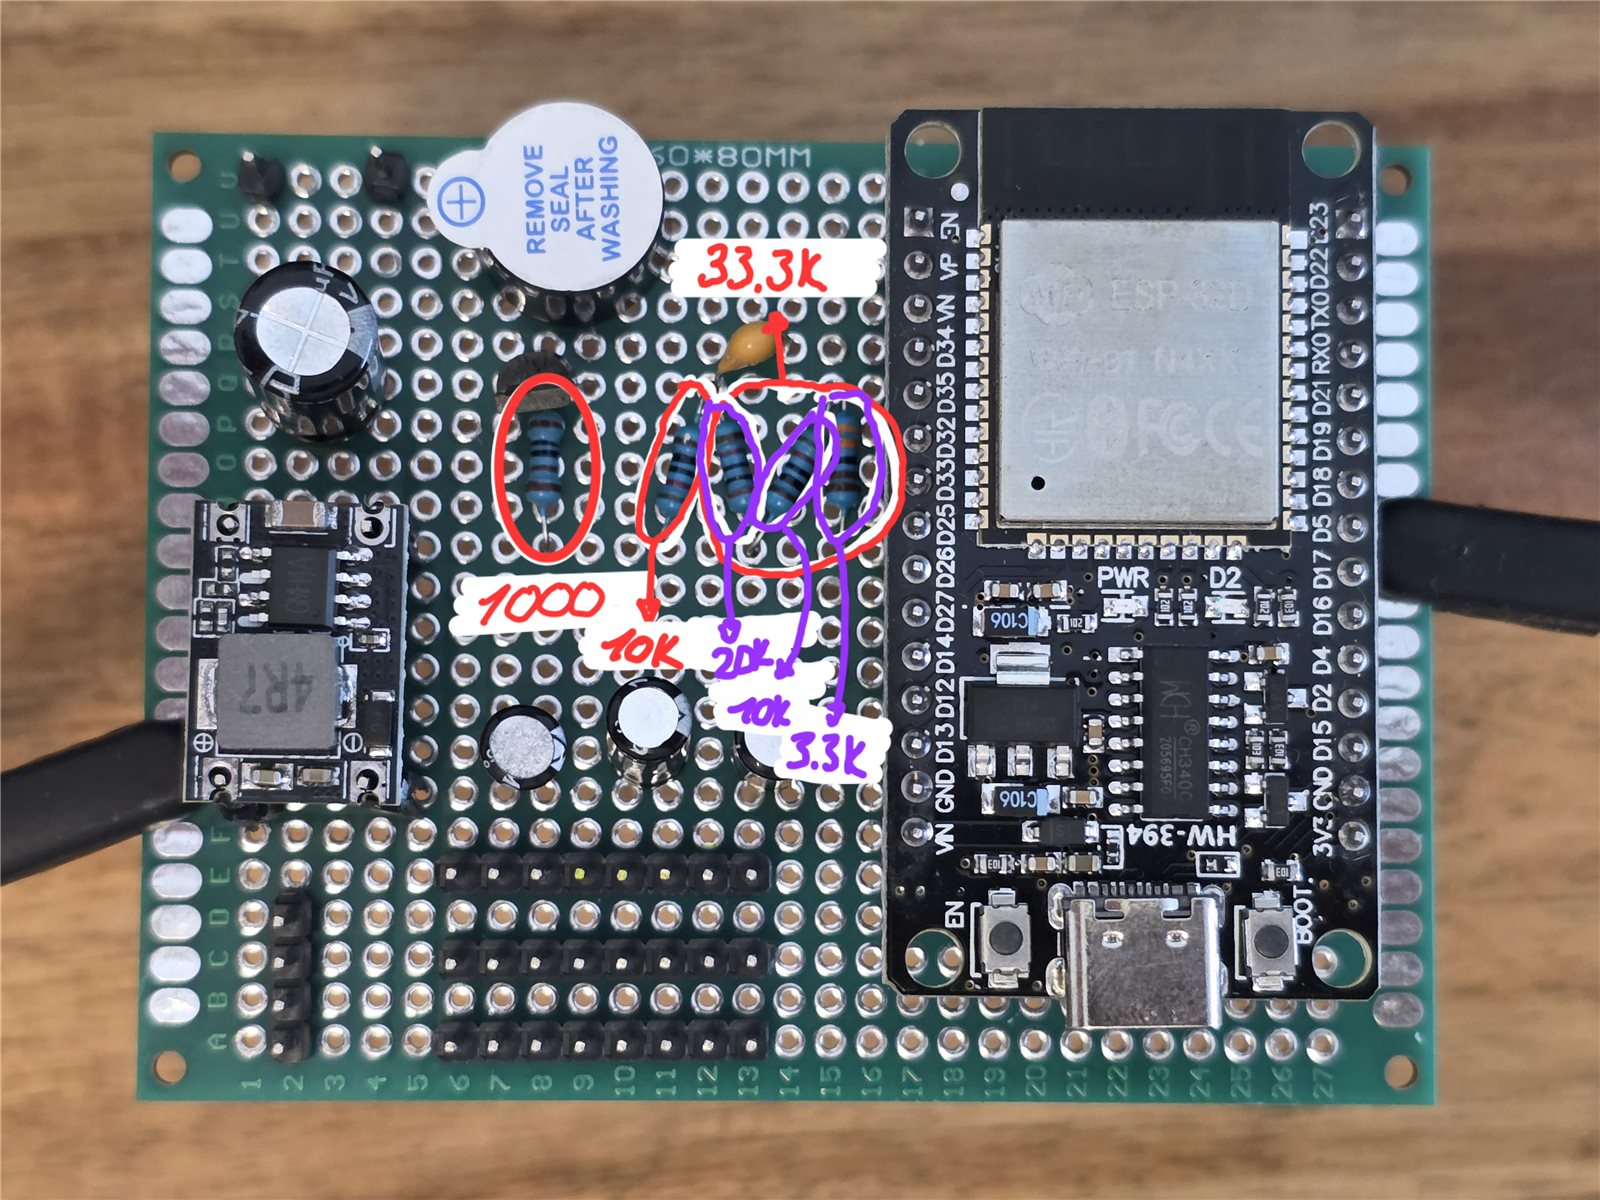
\includegraphics[width=\textwidth]{pcb_top_view_annotated.jpg}
    \caption{Top side with the resistor values marked.}
    \label{fig:pcb_top}
  \end{subfigure}\hfill
  \begin{subfigure}[b]{0.49\textwidth}
    \centering
    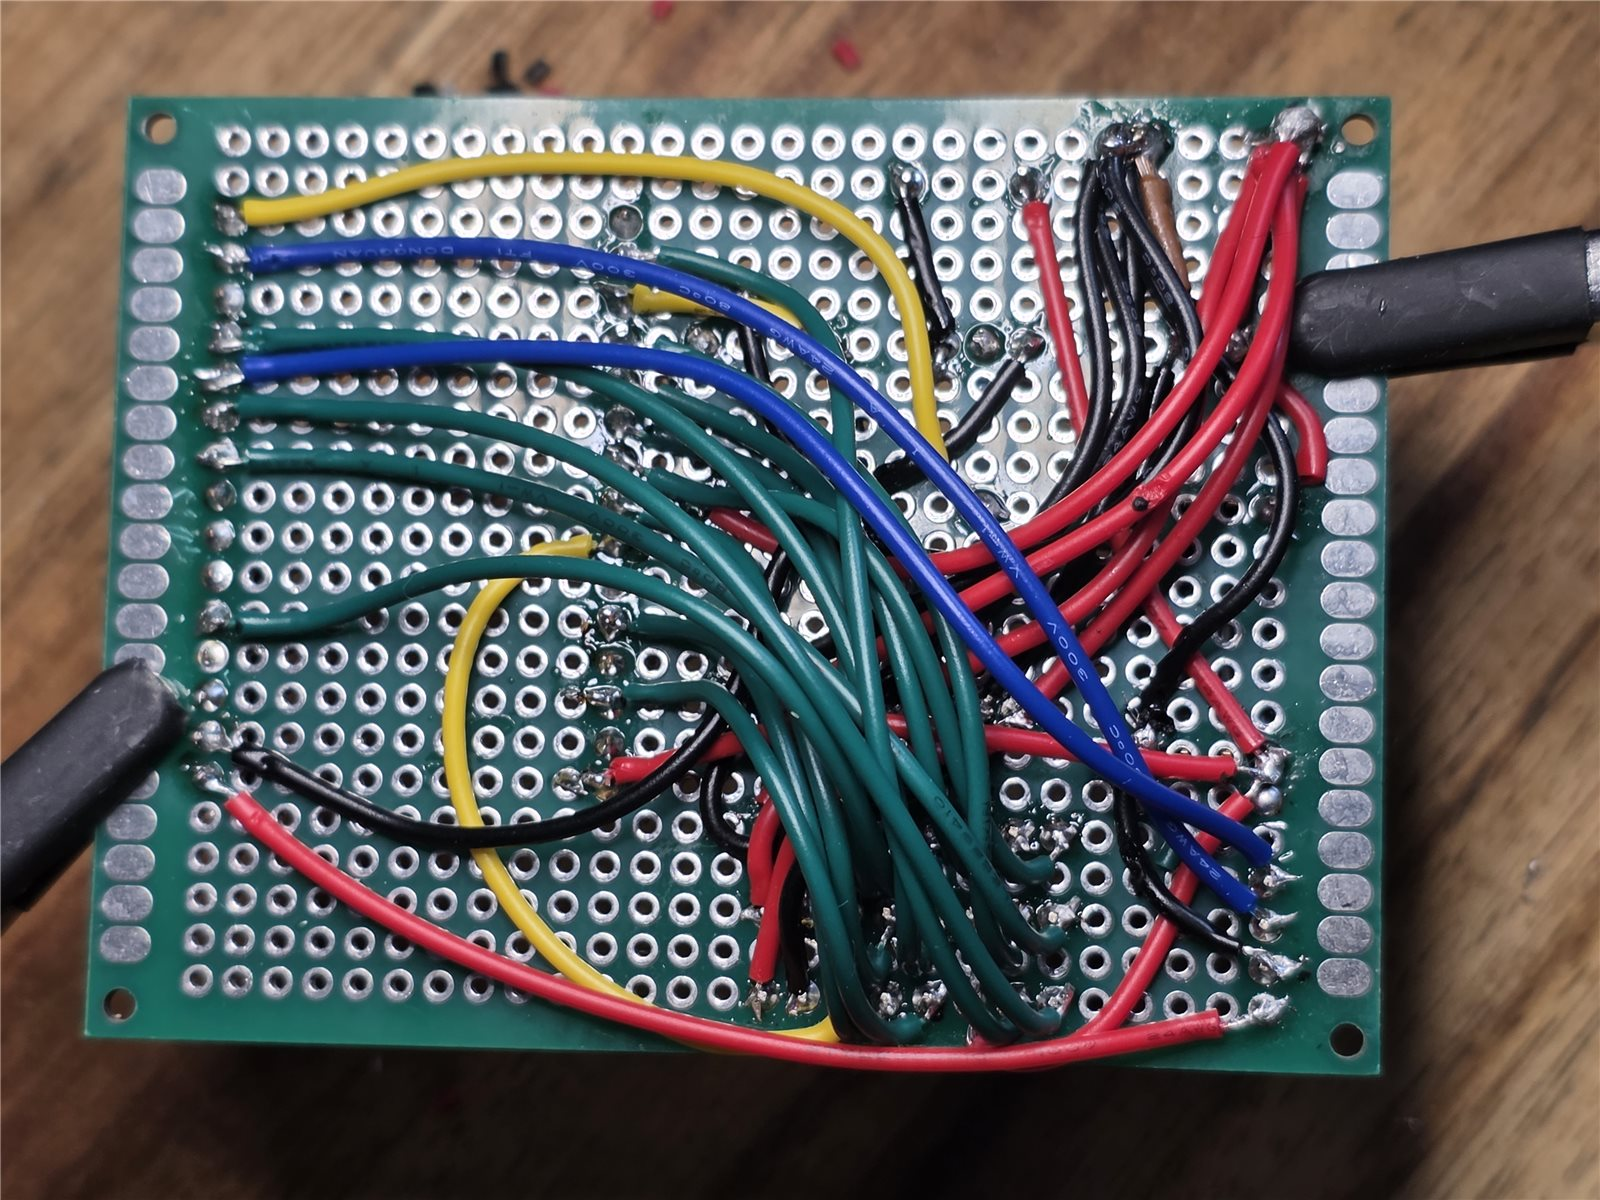
\includegraphics[width=\textwidth]{pcb_bottom_view_wiring.jpg}
    \caption{Bottom side with the colour-coded wiring.}
    \label{fig:pcb_bottom}
  \end{subfigure}
  \caption{The prototype board: ESP32 board (right), buck converter (left), buzzer, voltage
    divider, buffer capacitors and the pin headers for the motors and the IMU.}
  \label{fig:pcb}
\end{figure}

The motor cables were extended with ordinary jumper wires with \SI{2.54}{mm} female connectors,
soldered to the motor wires and insulated with heat shrink tubing (\cref{fig:wiring_extension}).
This takes some time but is cheap and works well. Alternatives are ready-made extension cables
or crimping 8-pin cables with a matching connector kit.

\begin{figure}[htbp]
  \centering
  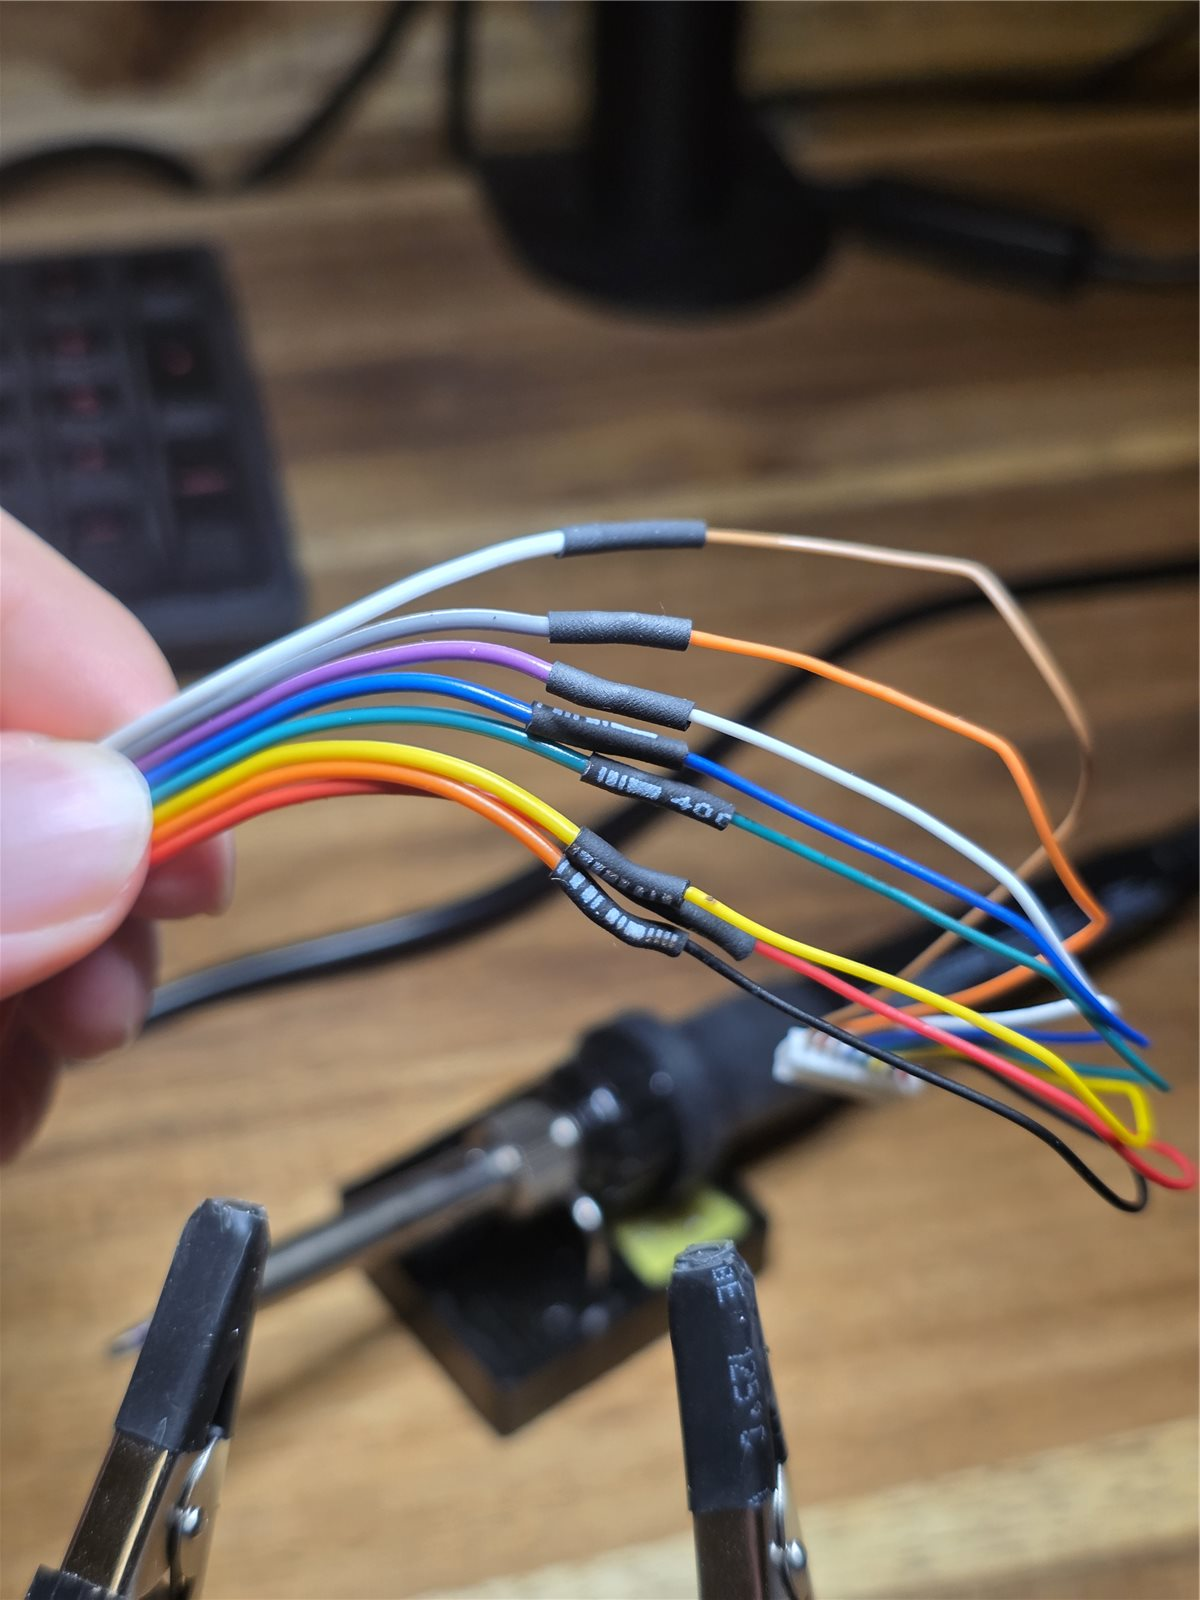
\includegraphics[width=0.45\textwidth]{soldered_wiring_extension.jpg}
  \caption{Motor cable extended with jumper wires, insulated with heat shrink tubing.}
  \label{fig:wiring_extension}
\end{figure}

\section{Safety note on the battery connection}

The XT30 battery connector is soldered to the board via pin headers. These contacts are not
insulated. They were useful during testing for measuring the battery voltage with a multimeter,
but they are dangerous: touching them or accidentally bridging them causes a short circuit of the
LiPo battery. \textbf{Do not copy this detail}; insulate all battery contacts.

\chapter{Firmware and Control}
\label{ch:firmware}

The firmware is written in C++ for the Arduino core for the ESP32~\cite{arduino_esp32} and uses
the MPU6050\_light library~\cite{mpu6050light} to read the IMU. This chapter explains its structure
and the control laws. The firmware is located in the folder \cmd{firmware/cubilox\_mk1/}.

\section{Source files}

\begin{table}[htbp]
  \centering
  \caption{Source files of the firmware.}
  \label{tab:files}
  \begin{tabularx}{\textwidth}{lX}
    \toprule
    File & Content \\
    \midrule
    \cmd{cubilox\_mk1.ino} & \cmd{setup()} and \cmd{loop()}: start-up, sensor filters, state
      machine, edge and vertex controllers \\
    \cmd{config.h} & pin definitions, controller gains, limits and timing constants, shared state
      variables \\
    \cmd{calibration.ino} & gyroscope calibration at start-up, edge and vertex calibration,
      storage in flash, pose detection \\
    \cmd{commands.ino} & command interface over USB and Bluetooth, storage of the gains \\
    \cmd{hardware.ino} & log output, battery measurement, buzzer, motor control, encoder
      interrupts, motor test \\
    \bottomrule
  \end{tabularx}
\end{table}

The Arduino IDE combines all \cmd{.ino} files of the sketch folder into one program; global
variables shared between the files are therefore declared in \cmd{config.h}.

\section{Start-up}

\cmd{setup()} performs the following steps:
\begin{enumerate}
  \item start the USB serial port (\SI{115200}{baud}) and Bluetooth with the device name
        \cmd{Cubilox\_Mk1},
  \item load the gains and the calibration from flash,
  \item configure the pins, attach the PWM outputs (\SI{20}{kHz}, 8~bit) and the encoder
        interrupts, stop all motors and engage the brake,
  \item initialise the IMU (gyroscope range \SI{\pm 500}{\degree/s}, accelerometer range
        \SI{\pm 2}{g}, the defaults of the library),
  \item calibrate the gyroscope (the cube must lie still, see \cref{sec:calibration}),
  \item measure the battery voltage and report the calibration status.
\end{enumerate}
After that, the cube waits until it is placed on a calibrated edge or vertex and starts balancing
automatically.

\section{Main loop and timing}

\cmd{loop()} runs continuously. In every pass it processes incoming commands, reads the IMU and
updates the sensor filters. The controllers themselves run whenever at least \SI{5}{ms} have
passed since the last control step, i.e.\ at up to \SI{200}{Hz}. The debug output reports the
longest gap between two control steps (\cmd{loop=}); on the real cube it is \SIrange{5}{6}{ms}.

The wheel speeds are computed from the encoder counts in a window of \SI{20}{ms} and scaled by 5,
so that their unit is \enquote{encoder counts per \SI{100}{ms}}. All wheel speeds and wheel
momenta in this chapter use this unit.

\section{State machine}
\label{sec:state_machine}

The firmware has three states:
\begin{description}
  \item[WAITING] The motors are off and braked. The firmware compares the measured acceleration
    vector with the calibrated edge and vertex poses. If it is closer than \SI{0.25}{g} to one of
    them, the cube is close enough to the balance point (edge: $|\theta| < \ang{1}$, vertex:
    tilt $< \ang{1.5}$), it is at rest ($\left||\vect{a}| - \SI{1}{g}\right| < \SI{0.3}{g}$), the
    battery is not empty and these conditions hold for \SI{400}{ms}, the brake is released and the
    corresponding balancing state is entered.
  \item[RUNNING\_EDGE] The edge controller drives motor X. The motor command is ramped up over
    \SI{800}{ms}. Balancing stops if the angle exceeds \ang{15} or the cube is moved
    ($\left||\vect{a}| - \SI{1}{g}\right| > \SI{0.3}{g}$).
  \item[RUNNING\_VERTEX] The vertex controller drives all three motors. The command is ramped up
    over \SI{150}{ms}. Balancing stops if the tilt exceeds \ang{25}, if a shock
    ($\left||\vect{a}| - \SI{1}{g}\right| > \SI{1.2}{g}$) lasts longer than \SI{150}{ms}, or if at
    least one motor command stays above the maximum of 255 for more than \SI{200}{ms}
    (saturation).
\end{description}
When balancing stops, all motors are switched off and braked, the run time and the cause are
reported, and the state returns to WAITING.

\section{Sensor processing}
\label{sec:sensor_processing}

\subsection{Edge angle}

On the edge, only the rotation about the sensor's X axis matters. The firmware uses the X tilt
angle $\varphi_x$ computed by the MPU6050\_light library, subtracts the calibrated offset
$\varphi_0$ and combines it with the gyroscope rate $\omega_x$ in a complementary filter:
\begin{equation}
  \theta_k = 0.98\left(\theta_{k-1} + \omega_x\,\Delta t\right) + 0.02\left(\varphi_x - \varphi_0\right).
  \label{eq:edge_cf}
\end{equation}
Here $\Delta t$ is the time since the last control step, not since the last filter step. The edge
gains were tuned with this behaviour, so it was deliberately left unchanged.

\subsection{Vertex tilt vector}

On the vertex, the tilt is a three-dimensional vector. The current gravity direction $\vect{n}$ is
the normalised accelerometer vector, $\vect{r}$ the normalised calibrated vertex pose. The
accelerometer-based tilt error (in degrees) is
\begin{equation}
  \vect{e}_\text{acc} = \frac{180}{\pi}\,\left(\vect{n}\times\vect{r}\right).
\end{equation}
The order of the cross product matters: $\vect{n}\times\vect{r}$ has the same sign as the
integrated gyroscope rate (with the MPU6050\_light conventions, a positive rotation about X
increases the measured Y acceleration). The opposite order was the main bug during development
(\cref{sec:history}).

The tilt estimate $\vect{e}$ is obtained with a complementary filter with the time constant
$\tau = \SI{0.5}{s}$:
\begin{equation}
  \vect{e}_k = a\left(\vect{e}_{k-1} + \vect{\omega}\,\Delta t\right) + (1-a)\,\vect{e}_\text{acc},
  \qquad a = \frac{\tau}{\tau + \Delta t},
  \label{eq:vertex_cf}
\end{equation}
where $\vect{\omega}$ is the gyroscope rate vector and $\Delta t$ the measured time since the last
filter step. The long time constant suppresses the disturbances of the accelerometer caused by the
wheel accelerations. After every filter step, the component of $\vect{e}$ along $\vect{r}$ is
removed, because a rotation about the vertical axis is not a tilt and is never corrected by the
accelerometer.

\section{Edge controller}
\label{sec:edge_controller}

The edge controller implements \cref{eq:edge_law} for motor X:
\begin{equation}
  u_X = \rho(t)\,\Bigl(k_{e1}\,(\theta - \theta_\text{trim}) + k_{e2}\,\omega_x + k_{e3}\,n_X\Bigr),
  \label{eq:edge_controller}
\end{equation}
with the gains $k_{e1}$, $k_{e2}$, $k_{e3}$ (\cmd{ek1}, \cmd{ek2}, \cmd{ek3}), the wheel speed
$n_X$ of motor X and the start-up ramp $\rho(t)$ that rises linearly from 0 to 1. The command
$u_X$ is limited to $\pm 255$.

\begin{lstlisting}[caption={Edge controller in \cmd{cubilox\_mk1.ino}.}, label={lst:edge}]
float output = (eK1 * edgeAngle + eK2 * gyroRateX + eK3 * motorSpeed_X) * rampFactor;
motorControl_X((int)output);
\end{lstlisting}

\subsection{Automatic trim}
\label{sec:trim}

If the calibrated balance point is slightly off, the wheel keeps turning in one direction
(\cref{sec:wheel_speed}). According to \cref{eq:equilibrium}, a positive wheel speed means that the
angle setpoint is too large. The trim therefore moves the setpoint slowly against the wheel speed:
\begin{equation}
  \theta_\text{trim} \leftarrow \theta_\text{trim} - k_\text{trim}\, n_X\, \Delta t ,
\end{equation}
limited to \SI{\pm 3}{\degree}, with the rate $k_\text{trim}$ (\cmd{trim}, default 0.001). The trim
is only active after the start-up ramp and is kept after a fall. On the real cube, the wheel
oscillates around zero and the trim stays within about \SI{\pm 0.1}{\degree}.

\section{Vertex controller}
\label{sec:vertex_controller}

The vertex controller works in the coordinate frame of the cube. The motors Y and Z are mounted
mirrored, which is described by the motor signs $s = (+1, -1, -1)$ and the encoder signs
$w = (+1, +1, +1)$ in \cmd{config.h}. The physical wheel momentum vector is
\begin{equation}
  \vect{h} = \bigl(s_X w_X n_X,\; s_Y w_Y n_Y,\; s_Z w_Z n_Z\bigr).
\end{equation}
Both the gyroscope rate $\vect{\omega}$ and the wheel momentum $\vect{h}$ are split into a tilt part
and a yaw part according to \cref{eq:split}. The torque command vector is
\begin{equation}
  \vect{t} = k_{v1}\,(\vect{e} - \vect{e}_\text{trim}) + k_{v2}\,\vect{\omega}_\text{tilt}
           + k_{v3}\,\vect{h}_\text{tilt}
           + \bigl(k_{yd}\,\omega_\text{yaw} - k_{yw}\,h_\text{yaw}\bigr)\,\vect{r},
  \label{eq:vertex_controller}
\end{equation}
where $\omega_\text{yaw} = \vect{\omega}\cdot\vect{r}$ and $h_\text{yaw} = \vect{h}\cdot\vect{r}$.
The gains are \cmd{vk1}, \cmd{vk2}, \cmd{vk3} for the tilt and \cmd{vyd}, \cmd{vyw} for the yaw
axis. The three motor commands are
\begin{equation}
  u_i = \rho(t)\, s_i\, t_i ,\qquad i \in \{X, Y, Z\}.
\end{equation}
The first three terms of \cref{eq:vertex_controller} are the three-dimensional version of the edge
controller. The yaw term damps the rotation about the vertical axis and slowly removes the yaw
momentum of the wheels; $k_{yw}$ must be positive, otherwise it is a positive feedback
(\cref{sec:yaw_physics}).

\begin{lstlisting}[caption={Core of the vertex controller in \cmd{cubilox\_mk1.ino}.},
  label={lst:vertex}]
float yawTorque = vYawD * gYaw - vYawW * hYaw;
float tX = vK1 * (cfVertexAngleX - vTrimX) + vK2 * gTx + vK3 * hTx + yawTorque * rx;
float tY = vK1 * (cfVertexAngleY - vTrimY) + vK2 * gTy + vK3 * hTy + yawTorque * ry;
float tZ = vK1 * (cfVertexAngleZ - vTrimZ) + vK2 * gTz + vK3 * hTz + yawTorque * rz;

float outX = MOTOR_SIGN_X * tX * rampFactor;
float outY = MOTOR_SIGN_Y * tY * rampFactor;
float outZ = MOTOR_SIGN_Z * tZ * rampFactor;
\end{lstlisting}

The vertex has an automatic trim as well, which works like the edge trim but as a vector
perpendicular to $\vect{r}$:
$\vect{e}_\text{trim} \leftarrow \vect{e}_\text{trim} - k_\text{vtrim}\,\vect{h}_\text{tilt}\,\Delta t$,
limited to \ang{3}. Its rate \cmd{vtrim} is 0 (off) by default, because the cube balances best
with a careful calibration by hand (\cref{sec:history}).

\section{Calibration and persistent storage}
\label{sec:calibration}

\subsection{Gyroscope}

The gyroscope has a small offset that changes with temperature. It is therefore measured at every
start: the cube only has to lie still for about three seconds. The surface does not need to be
level, because only the gyroscope is calibrated.

\subsection{Edge and vertex poses}

The balance points of the edge and the vertex are measured once with the commands \cmd{edge} and
\cmd{vertex} and stored in flash. The user balances the cube by hand on the edge or vertex;
after \SI{7}{s} (one short tick per second), the acceleration vector is averaged for \SI{3}{s}.
The measurement is rejected if
\begin{itemize}
  \item the standard deviation of one acceleration component exceeds \SI{0.05}{g} (the cube was
        moved), or
  \item the measured direction is more than \ang{12} away from an ideal pose: for the vertex a
        space diagonal $(\pm 1, \pm 1, \pm 1)/\sqrt{3}$, for the edge a diagonal in the Y--Z plane,
        i.e.\ an edge parallel to the axis of motor X.
\end{itemize}

Balancing by hand finds the \emph{real} balance point, where the centre of mass is exactly above
the pivot. A fixture that holds the cube geometrically straight does not, because the centre of
mass is generally not exactly in the geometric centre. This difference was the key to stable vertex
balancing (\cref{sec:history}).

The accelerometer offsets are not recomputed at start-up. The offsets that were active during the
calibration are stored together with the poses and loaded again at every start, so that the
stored poses remain valid after every restart and power loss. (A constant accelerometer offset does
not matter for balancing, because the poses are measured with the same offset.)

\begin{table}[htbp]
  \centering
  \caption{Data stored in the flash memory (ESP32 \cmd{Preferences}).}
  \label{tab:flash}
  \begin{tabularx}{\textwidth}{llX}
    \toprule
    Namespace & Content & Deleted by \\
    \midrule
    \cmd{cube}    & controller gains (after \cmd{save}) & \cmd{reset} \\
    \cmd{cuberef} & edge and vertex poses, accelerometer offsets & new calibration (overwrites) \\
    \cmd{cubebat} & battery voltage factor (after \cmd{vbatcal}) & new \cmd{vbatcal} \\
    \bottomrule
  \end{tabularx}
\end{table}

\section{Communication and logging}

Commands can be sent over the USB serial port or over Bluetooth Classic (serial port profile) with
any serial terminal; they are listed in \cref{sec:commands}. All output goes to both interfaces.

During development, an analysis of the Bluetooth library showed that it sends every print call
as a separate packet; with a connected client, its transmit queue holds 32 packets and a full
queue can block the caller for up to one second. Since the diagnostic output consisted of many
print calls, this could stall the control loop. The firmware therefore formats each log line completely and
sends it as one packet (\cmd{logLine()}), and it always writes the motor commands \emph{before}
any log output.

In normal operation, the cube only reports the start and the end of a balancing run (with the run
time and the cause) and a short status line every \SI{10}{s}. With \cmd{debug 1}, detailed lines
are printed (\cref{tab:debug}).

\begin{table}[htbp]
  \centering
  \caption{Debug output (\cmd{debug 1}).}
  \label{tab:debug}
  \begin{tabularx}{\textwidth}{lX}
    \toprule
    Line & Fields \\
    \midrule
    \cmd{IDLE} (every \SI{500}{ms}) & detected pose, acceleration vector, edge angle, vertex tilt,
      battery voltage \\
    \cmd{EDGE} (every \SI{500}{ms}) & time \cmd{t}, \cmd{angle}, wheel speed \cmd{wheel}, \cmd{trim},
      longest control gap \cmd{loop} \\
    \cmd{RUN} (every \SI{50}{ms}) & time \cmd{t}, tilt vector \cmd{e}, gyroscope \cmd{g}, wheel
      speeds \cmd{w}, motor commands \cmd{o}, yaw and tilt momentum, trim vector, \cmd{loop} \\
    \cmd{STOP} & tilt, acceleration magnitude and number of short shocks at the end of a vertex run \\
    \bottomrule
  \end{tabularx}
\end{table}

\section{Where to change what}

Most settings are constants in \cmd{config.h}:
\begin{itemize}
  \item \textbf{Pins} (\cmd{PWM\_X}, \cmd{DIR\_X}, \ldots): adapt them if the board is wired
        differently.
  \item \textbf{Default gains} (\cmd{eK1}--\cmd{eK3}, \cmd{vK1}--\cmd{vK3}, \cmd{vYawD},
        \cmd{vYawW}, trim rates): they are used until gains are stored with \cmd{save}.
  \item \textbf{Motor and encoder signs} (\cmd{MOTOR\_SIGN\_*}, \cmd{WHEEL\_SIGN\_*}): must match
        the mounting direction of the motors; the command \cmd{motortest} recommends them.
  \item \textbf{Start and stop limits} (\cmd{EDGE\_START\_ANGLE\_DEG},
        \cmd{VERTEX\_STOP\_ANGLE\_DEG}, ramp times, \cmd{SATURATION\_STOP\_MS}, \ldots).
  \item \textbf{Calibration timing} (\cmd{CALIB\_SETTLE\_MS} = \SI{7}{s},
        \cmd{CALIB\_AVERAGE\_MS} = \SI{3}{s}) and its plausibility limits.
  \item \textbf{Battery} (\cmd{VBAT\_FACTOR}, \cmd{BAT\_WARN\_V}, \cmd{BAT\_MIN\_V}).
  \item \textbf{Bluetooth name} (\cmd{BT\_DEVICE\_NAME}).
\end{itemize}

\chapter{Getting Started}
\label{ch:getting_started}

This chapter describes how to flash the firmware, start the cube for the first time and calibrate
it.

\section{Software requirements}

\begin{itemize}
  \item Arduino IDE~2,
  \item Arduino core for the ESP32~\cite{arduino_esp32}, version 3.x (tested with 3.3.10;
        installed through the Boards Manager),
  \item library MPU6050\_light~\cite{mpu6050light} (tested with 1.2.1; installed through the
        Library Manager).
\end{itemize}
The libraries \cmd{BluetoothSerial}, \cmd{Preferences} and \cmd{Wire} are part of the ESP32 core.

\section{Flashing the firmware}

\begin{enumerate}
  \item Open \cmd{firmware/cubilox\_mk1/cubilox\_mk1.ino} in the Arduino IDE. The folder name must
        match the name of the main file, so do not rename it.
  \item Select the board \enquote{ESP32 Dev Module} and the default partition scheme (Bluetooth
        needs the default scheme; the firmware uses about \SI{85}{\percent} of the program memory).
  \item Connect the ESP32 via USB and upload the sketch.
\end{enumerate}
With the Arduino command line tool, the equivalent command is
\begin{lstlisting}[language=bash, numbers=none]
arduino-cli compile --fqbn esp32:esp32:esp32 firmware/cubilox_mk1
arduino-cli upload  --fqbn esp32:esp32:esp32 -p <port> firmware/cubilox_mk1
\end{lstlisting}

\section{Connecting}

Commands can be sent in two ways:
\begin{itemize}
  \item \textbf{USB:} serial monitor of the Arduino IDE, \SI{115200}{baud}, line ending
        \enquote{newline}. The USB cable disturbs the balance, so this is mainly useful on the
        desk.
  \item \textbf{Bluetooth:} pair the device \cmd{Cubilox\_Mk1} and use a serial terminal app, for
        example \enquote{Serial Bluetooth Terminal} on Android. The ESP32 uses Bluetooth Classic
        (serial port profile), which iPhones do not support.
\end{itemize}

\section{First start}

\begin{enumerate}
  \item Charge the battery fully and connect it.
  \item Lay the cube on any side and do not touch it. After a short beep it calibrates the
        gyroscope (about \SI{3}{s}), then two beeps follow, and a long beep signals that it is ready.
  \item Connect via Bluetooth and send \cmd{status}. On the first start, it reports that the edge
        and the vertex are not calibrated.
  \item Optional: run \cmd{motortest} while holding the cube loosely in your hand. All three
        encoder values should be similar (about 380 on the original cube) and the recommended
        signs should match \cmd{config.h}.
  \item \textbf{Calibrate the edge:} send \cmd{edge}. Within \SI{7}{s}, balance the cube by hand on
        an edge that is parallel to the axis of motor X, as still as possible. A long beep starts
        the measurement; hold the cube still for \SI{3}{s}. Two beeps confirm the calibration.
  \item \textbf{Calibrate the vertex:} send \cmd{vertex} and do the same on the vertex. Find the
        point where the cube balances by itself with almost no force from your fingers.
  \item Place the cube on the edge or vertex and hold it gently near the balance point. When it
        detects the pose, it starts by itself (two short beeps).
\end{enumerate}
The calibration is stored permanently. It only has to be repeated if something changes the
centre of mass, for example if the battery is mounted in a different position. If the vertex
balance is restless or the cube drifts away in one direction, a new \cmd{vertex} calibration
usually helps; several attempts may be needed to find the best balance point.

\section{Beep signals}

\begin{table}[htbp]
  \centering
  \caption{Beep signals of the buzzer.}
  \label{tab:beeps}
  \begin{tabularx}{\textwidth}{lX}
    \toprule
    Signal & Meaning \\
    \midrule
    1 short beep at power-on & IMU found, gyroscope calibration follows \\
    2 beeps, then 1 long beep & gyroscope calibrated, cube ready \\
    2 short beeps & balancing started \\
    1 beep (\SI{200}{ms}) & balancing stopped \\
    1 beep, then ticks every second & calibration: balance the cube now \\
    1 long beep (\SI{150}{ms}) during calibration & measurement starts, hold still \\
    2 beeps after calibration & calibration saved \\
    1 very long beep (\SI{800}{ms}) & calibration rejected \\
    3 short beeps (every \SI{30}{s}) & battery low (below \SI{11.1}{V}) \\
    1 beep every \SI{2}{s} when placed on a pose & battery empty (below \SI{10.5}{V}), no start \\
    1-second beep every \SI{2}{s} after power-on & IMU not found \\
    \bottomrule
  \end{tabularx}
\end{table}

\section{Commands}
\label{sec:commands}

\begin{table}[H]
  \centering
  \caption{Commands (USB or Bluetooth, one command per line).}
  \label{tab:commands}
  \begin{tabularx}{\textwidth}{lX}
    \toprule
    Command & Function \\
    \midrule
    \cmd{help} or \cmd{?} & list of commands \\
    \cmd{status} or \cmd{p} & current gains, calibration status, battery voltage, debug mode \\
    \cmd{edge} & calibrate the edge balance point (\cref{sec:calibration}) \\
    \cmd{vertex} & calibrate the vertex balance point \\
    \cmd{<gain> <value>} & set a gain, e.g.\ \cmd{vk1 95} (see \cref{ch:tuning}) \\
    \cmd{<gain>} & show a gain \\
    \cmd{save} & store all gains in flash \\
    \cmd{reset} & delete the stored gains and use the defaults from \cmd{config.h} \\
    \cmd{debug 0} / \cmd{debug 1} & detailed log output off / on \\
    \cmd{motortest} & short pulse on each motor; shows gyroscope reaction, encoder counts and the
      recommended motor and encoder signs \\
    \cmd{vbatcal <V>} & optional: fine-tune the battery measurement to a multimeter reading, e.g.\
      \cmd{vbatcal 12.6} \\
    \bottomrule
  \end{tabularx}
\end{table}
Commands that write to flash or move the motors (\cmd{edge}, \cmd{vertex}, \cmd{save},
\cmd{reset}, \cmd{motortest}, \cmd{vbatcal}) are only accepted while the cube is not balancing.
Changed gains are lost at the next restart unless they are stored with \cmd{save}.

\chapter{Tuning Guide}
\label{ch:tuning}

The gains can be changed at runtime over Bluetooth (for example \cmd{vk2 9}) and stored with
\cmd{save}. \Cref{tab:gains} lists all gains with their default values, which are the values the
cube balances with. The motor command is a PWM value between $-255$ and $+255$; angles are in
degrees, rates in degrees per second and wheel speeds in encoder counts per \SI{100}{ms}.

\begin{table}[htbp]
  \centering
  \caption{Tunable gains and their default values.}
  \label{tab:gains}
  \begin{tabularx}{\textwidth}{llX}
    \toprule
    Command & Default & Meaning \\
    \midrule
    \cmd{ek1}   & 70    & edge: angle gain (PWM per degree) \\
    \cmd{ek2}   & 8     & edge: rate gain (PWM per degree/s) \\
    \cmd{ek3}   & 0.35  & edge: wheel speed gain \\
    \cmd{trim}  & 0.001 & edge: rate of the automatic trim (0 = off) \\
    \cmd{vk1}   & 90    & vertex: tilt angle gain \\
    \cmd{vk2}   & 9.5   & vertex: tilt rate gain \\
    \cmd{vk3}   & 0.30  & vertex: wheel momentum gain (tilt part) \\
    \cmd{vyd}   & 9.5   & vertex: damping of the rotation about the vertical axis \\
    \cmd{vyw}   & 0.15  & vertex: reduction of the wheel momentum about the vertical axis \\
    \cmd{vtrim} & 0     & vertex: rate of the automatic trim (0 = off) \\
    \bottomrule
  \end{tabularx}
\end{table}

\section{Effect of the gains}

\begin{description}
  \item[Angle gain (\cmd{ek1}, \cmd{vk1})] determines how strongly the cube is pushed back towards
    the balance point. Too low: the cube reacts sluggishly, leans far and falls slowly to one side.
    Too high: it overreacts, oscillates quickly and the motors reach their limit.
  \item[Rate gain (\cmd{ek2}, \cmd{vk2})] damps the motion. Too low: the cube overshoots and
    oscillates. Too high: the motors react to sensor noise and switch rapidly back and forth; this
    is audible as a buzzing and produces short shocks. On the vertex, \cmd{vk2 11} caused such
    shocks, \cmd{vk2 9.5} did not.
  \item[Wheel speed gain (\cmd{ek3}, \cmd{vk3})] prevents the wheels from running away. Too low:
    the wheels slowly spin up until the motors saturate and the cube falls after a few seconds.
    Too high: a slow oscillation of the whole cube. During development, the vertex rocked slowly
    with a period of about \SI{1.3}{s} at 70\,/\,8\,/\,0.35; raising the angle and rate gains and
    slightly lowering the wheel gain (90\,/\,11\,/\,0.30, later 90\,/\,9.5\,/\,0.30) stabilised it.
  \item[Yaw damping (\cmd{vyd})] damps the rotation of the cube about its vertical axis.
  \item[Yaw momentum gain (\cmd{vyw})] slowly reduces the momentum of the wheels about the
    vertical axis. It \emph{must be positive}. With a negative value (\cmd{-0.3}), the yaw momentum
    grew exponentially until the motors saturated after 7--10\,s
    (\cref{sec:yaw_physics,sec:history}).
  \item[Trim rates (\cmd{trim}, \cmd{vtrim})] determine how fast the automatic trim corrects the
    balance point. The trim should be much slower than the balancing motion; a trim that is too
    fast can interact with the controller. On the vertex, a careful calibration by hand worked
    better than the trim, which is why \cmd{vtrim} is 0 by default.
\end{description}

\section{Recommended procedure}

\begin{enumerate}
  \item Start with a fully charged battery: the available motor power depends noticeably on the
        battery voltage.
  \item Calibrate first, then tune. Many problems that look like bad gains are actually a wrong
        balance point (\cref{sec:history}).
  \item Change only \textbf{one} gain at a time and test it several times. Changing two things at
        once made it impossible to tell which change caused an effect.
  \item Use \cmd{debug 1} and record the output. Check that every wheel speed (\cmd{w=}) reacts to
        its motor command (\cmd{o=}); a wheel that stays at zero indicates a hardware problem
        such as a loose connector.
  \item The cause reported at the end of a run helps: \enquote{motors saturated} usually means that
        the wheel speeds ran away (wheel speed gain, calibration or yaw gain),
        \enquote{tilt angle too large} that the cube fell over without the motors being at their
        limit (angle or rate gain), and \enquote{sustained shock} that the cube was hit or vibrates
        strongly.
  \item Store good values with \cmd{save}.
\end{enumerate}

\chapter{Assembly}
\label{ch:assembly}

The 3D files are published separately on MakerWorld (\href{https://makerworld.com/de/models/3406349-cubilox-mk1-self-balancing-cube-on-its-corner\#profileId-3879241}{Cubilox Mk1 on MakerWorld}). All parts
listed in \cref{tab:printed_parts} are printed in PLA; the author used a Bambu Lab A1 with the
default settings of Bambu Studio. The complete bill of materials is given in \cref{app:bom}.

\section{Reaction wheels and motors}

\begin{enumerate}
  \item Mount all M6 screws and nuts on the rims of the three flywheels first
        (\cref{fig:wheel}).
  \item Push each flywheel onto its motor shaft. The fit is very tight; on the original cube, the
        bore of the flywheel was widened slightly with drill bits until it fitted exactly.
  \item Clamp the flywheel to the shaft with the two hub screws. Make sure that the wheel sits
        exactly perpendicular on the shaft and does not wobble. A wobbling wheel causes
        vibrations and can rub against the frame.
  \item Screw the motor mounts to the motors with M4 screws and nuts.
\end{enumerate}

\section{Frame}

\begin{enumerate}
  \item Press the M3 nuts into the corner mounts. They should be a light press fit, so that they
        do not fall out during assembly.
  \item First assemble the three motor sides completely, then join the three sides using the
        corner mounts. This order makes the assembly much easier.
  \item If an M3 nut falls out, small tweezers help to put it back; with the fingers it is hard to
        reach.
\end{enumerate}

\section{Electronics}

\begin{enumerate}
  \item Solder the board according to the schematic (\cref{fig:schematic}) and
        \cref{tab:pins,tab:motor_pins}. Check all connections with a multimeter before connecting
        the battery for the first time.
  \item Extend the motor cables (\cref{fig:wiring_extension}) and connect them to the 8-pin
        headers, keeping the pin order.
  \item Mount the IMU on the sensor mount so that its X, Y and Z axes are parallel to the axes of
        motors X, Y and Z (\cref{fig:sensor_mount}).
  \item Pad the battery compartment (for example with cardboard and folded paper) so that the
        battery sits firmly and is protected against shocks.
  \item Insulate all battery contacts (see the safety note in \cref{ch:electronics}).
\end{enumerate}

\section{Commissioning}

Flash the firmware, run \cmd{motortest} and check the motor and encoder signs, then calibrate the
edge and the vertex as described in \cref{ch:getting_started}. If a motor of a rebuilt cube is
mounted in the opposite direction, the signs in \cmd{config.h} must be adapted to the values
recommended by \cmd{motortest}.

\chapter{Results}
\label{ch:results}

\section{Edge balancing}

The edge balancing works reliably. With the automatic trim, the wheel oscillates around zero speed
and the trim settles within about \SI{\pm 0.1}{\degree}. The cube also recovers from gentle pushes,
as shown in the animation in the repository (\cref{fig:edge_results}).

\begin{figure}[htbp]
  \centering
  \begin{subfigure}[b]{0.38\textwidth}
    \centering
    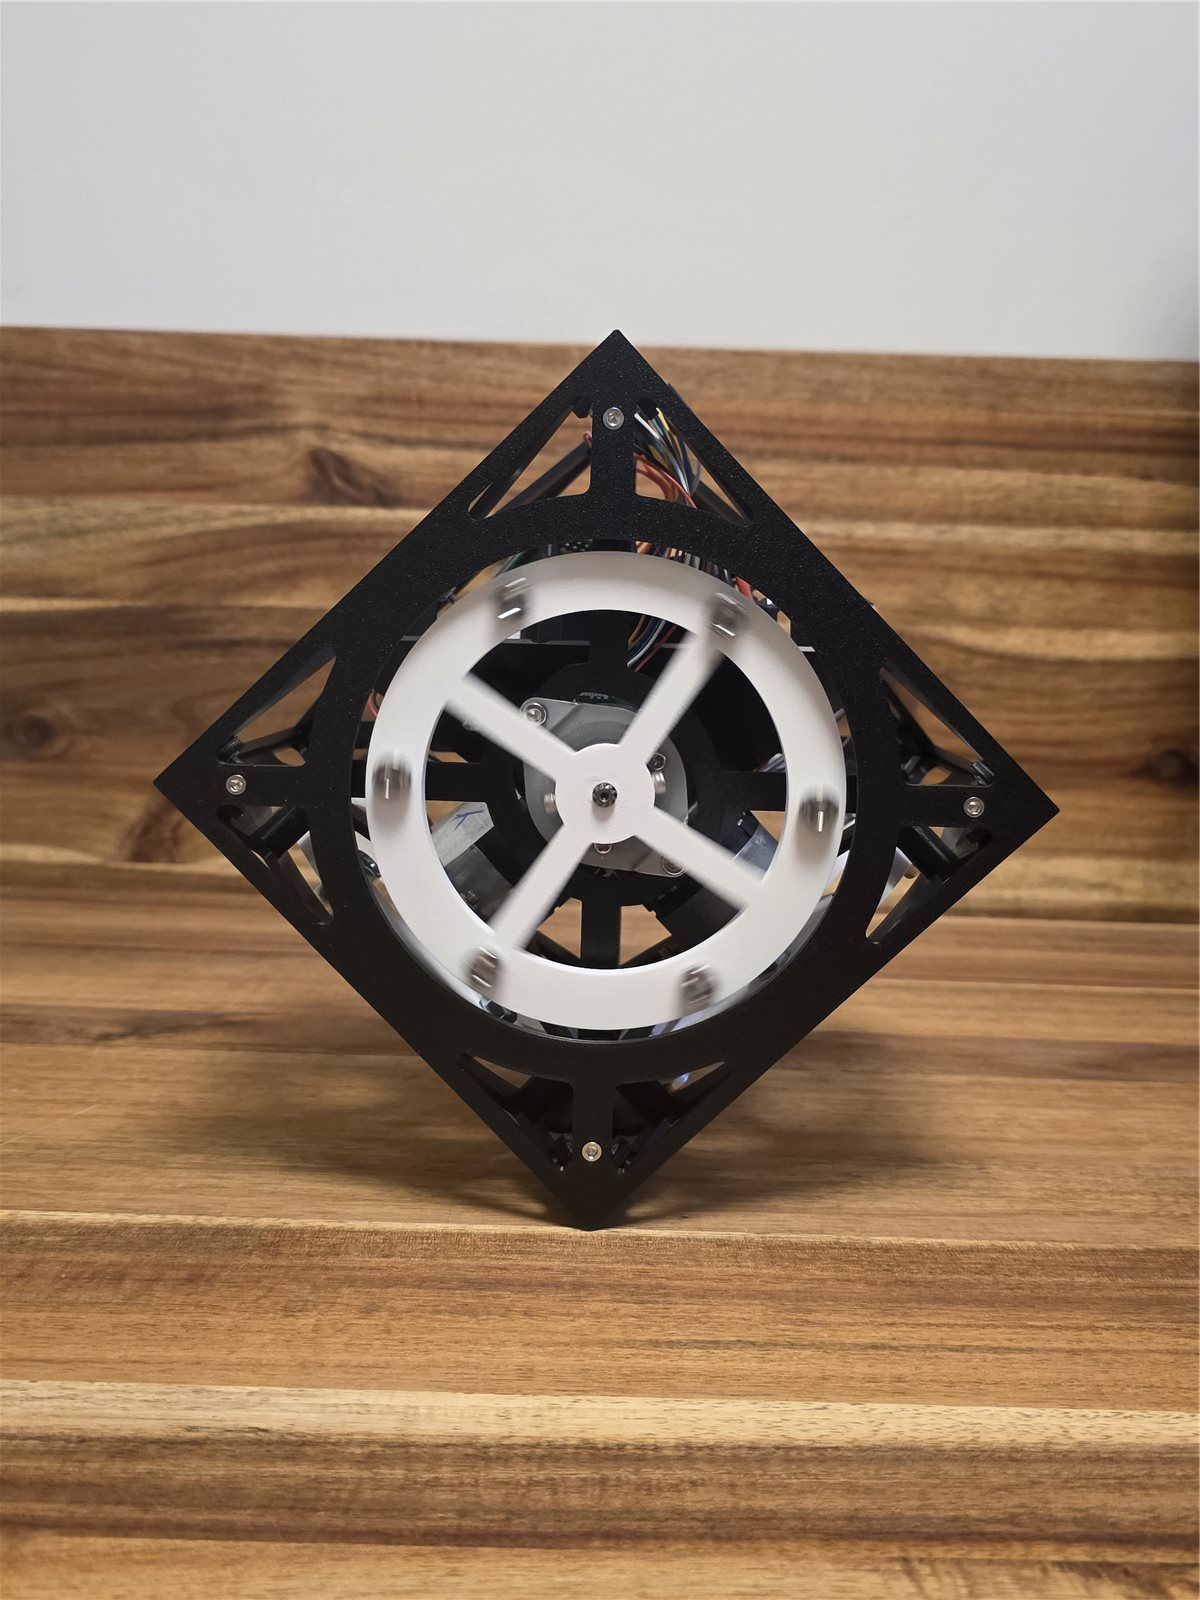
\includegraphics[width=\textwidth]{edge_balance_front_view.jpg}
    \caption{Front view of the cube balancing on its edge.}
    \label{fig:edge_front}
  \end{subfigure}\hspace{0.06\textwidth}
  \begin{subfigure}[b]{0.38\textwidth}
    \centering
    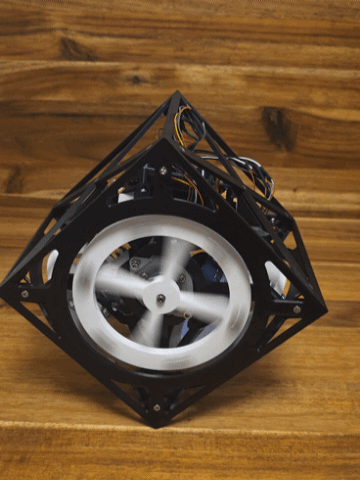
\includegraphics[width=\textwidth]{edge_balance_push_resistance_frame.png}
    \caption{Frame of the animation in which the cube is pushed while balancing on its edge.}
    \label{fig:edge_push}
  \end{subfigure}
  \caption{Balancing on the edge.}
  \label{fig:edge_results}
\end{figure}

\section{Vertex balancing}

After the improvements described in \cref{sec:history}, and in particular after calibrating the
vertex by hand, the cube balances on its vertex for several minutes in a row. Only a small residual
oscillation remains, which is attributed to the limited motor power and to a calibration that is
not perfect. \Cref{fig:vertex_results} shows frames of the two animations in the repository.

\begin{figure}[htbp]
  \centering
  \begin{subfigure}[b]{0.38\textwidth}
    \centering
    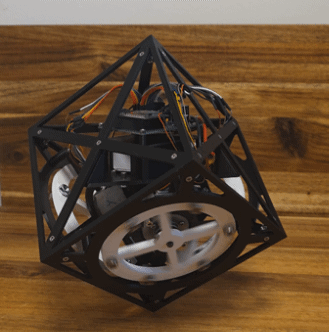
\includegraphics[width=\textwidth]{vertical_balance_loop_frame.png}
    \caption{Frame of the balancing loop animation.}
    \label{fig:vertex_loop}
  \end{subfigure}\hspace{0.06\textwidth}
  \begin{subfigure}[b]{0.38\textwidth}
    \centering
    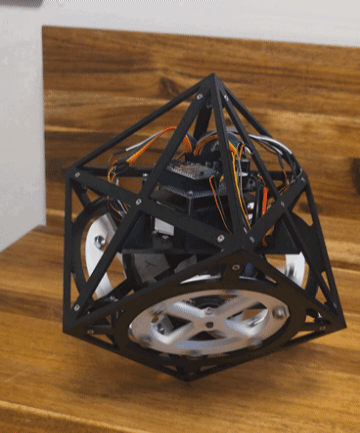
\includegraphics[width=\textwidth]{vertical_balance_around_view_frame.png}
    \caption{Frame of the animation with a view around the cube.}
    \label{fig:vertex_around}
  \end{subfigure}
  \caption{Balancing on the vertex.}
  \label{fig:vertex_results}
\end{figure}

\section{Motor test}

The motor test (\cmd{motortest}, PWM 150 for \SI{200}{ms}) gave encoder counts of 379, 377 and 380
for the motors X, Y and Z, confirming that the three motors deliver the same power, and the
measured gyroscope reactions confirmed the motor signs $(+1, -1, -1)$ and the encoder signs
$(+1, +1, +1)$.

\section{Development history and lessons learned}
\label{sec:history}

The vertex balancing did not work at the first attempt. \Cref{tab:history} summarises the most
important problems, their causes and the resulting balancing times on the vertex. Several of these
lessons apply to any balancing robot.

\begin{longtable}{>{\raggedright\arraybackslash}p{0.27\textwidth}>{\raggedright\arraybackslash}p{0.45\textwidth}>{\raggedright\arraybackslash}p{0.18\textwidth}}
  \caption{Development history of the vertex balancing.}
  \label{tab:history}\\
  \toprule
  Problem & Cause and solution & Vertex time \\
  \midrule
  \endfirsthead
  \toprule
  Problem & Cause and solution & Vertex time \\
  \midrule
  \endhead
  Vertex filter drifted to the wrong sign after about \SI{0.3}{s} &
    The tilt error was computed as $\vect{r}\times\vect{n}$ instead of $\vect{n}\times\vect{r}$,
    so gyroscope and accelerometer had opposite signs. Additionally, the filter used a wrong time
    step and included the yaw rotation. All three were fixed. & -- \\
  Cube slowly tipped away &
    The encoder signs of motors Y and Z were wrong, which cancelled half of the restoring
    action. Fixed with the motor test. & 1--2\,s \\
  Slow rocking with a period of about \SI{1.3}{s} &
    Gains changed from 70\,/\,8\,/\,0.35 to 90\,/\,11\,/\,0.30. & -- \\
  Motor Z stopped working in two runs &
    Loose contact (encoder showed zero despite a large command). & -- \\
  Run stopped by the shock detection although the cube was upright &
    Fast reversals of the wheels produced short accelerations above \SI{2}{g}; stopping and braking
    then threw the cube over. Now only a shock lasting longer than \SI{150}{ms} stops the run;
    \cmd{vk2} reduced to 9.5. & -- \\
  Cracking noises &
    A wheel rubbed against the frame because of a loose screw. & 7--8\,s \\
  Runs ended with the wheels saturated, cube visibly rotating about its vertical axis &
    The wheel momentum about the vertical axis was fed back like the tilt momentum (positive
    feedback). The yaw axis is now controlled separately (\cref{sec:yaw_physics}). & -- \\
  All run times suddenly much shorter (about \SI{2}{s}) &
    Bluetooth output blocked the control loop. Every log line is now sent as one packet, after the
    motor commands. Afterwards, the measured control gap was a constant \SI{6}{ms}. & 7--10\,s \\
  Results varied strongly between sessions &
    The vertex pose had been calibrated in a fixture that held the cube geometrically straight,
    but the centre of mass was slightly off the geometric axis. Calibrating by hand, at the real
    balance point, solved the problem. & several minutes \\
  \bottomrule
\end{longtable}

The main lessons are:
\begin{itemize}
  \item \textbf{Signs and conventions first.} Most early failures were sign errors. A motor test
        that measures the reaction of the cube to each motor saves a lot of time.
  \item \textbf{The balance point is defined by the centre of mass, not by the geometry.}
  \item \textbf{Look for positive feedback} when a quantity grows exponentially.
  \item \textbf{Logging must never block the control loop.}
  \item \textbf{Change only one thing at a time.} In one test series, two changes were made at
        once, and their effects could not be separated.
  \item \textbf{Mechanical problems look like control problems.} A rubbing wheel or a loose
        contact can ruin otherwise good gains.
\end{itemize}

\chapter{Limitations}
\label{ch:limitations}

The Cubilox Mk1 is the author's first large electronics project. It works, but several aspects
are not best practice or limit its performance:

\begin{itemize}
  \item \textbf{Motor power.} The available torque of the Nidec~24H motors is the main limit. Runs
        end when the motors saturate, a small residual oscillation remains on the vertex, and the
        cube cannot jump up by itself.
  \item \textbf{Empirical gains.} The gains were tuned by experiment. No model of the cube was
        identified, and no model-based controller (such as the linear state feedback of the
        Cubli~\cite{gajamohan2013cubli}) was designed.
  \item \textbf{Calibration by hand.} The vertex balance point has to be found by balancing the cube
        by hand; the result depends on the user and may need several attempts. The automatic
        vertex trim did not replace this calibration.
  \item \textbf{Edge balancing on one axis.} Only edges parallel to the axis of motor X are
        supported.
  \item \textbf{Sensor disturbances.} The accelerometer is disturbed by every wheel acceleration;
        the vertex filter therefore relies on the gyroscope for fast motion and corrects the tilt
        only slowly.
  \item \textbf{Prototype board.} All electronics are hand-wired on a prototype board. The wiring
        takes space, adds weight and is error-prone (one loose contact was found during
        development).
  \item \textbf{Exposed battery contacts.} The XT30 connector is attached via uninsulated pin
        headers, which is a short-circuit risk.
  \item \textbf{Schematic.} The schematic was the author's first KiCad project and is not as clearly
        laid out as it could be; two labels differ from the built cube
        (\cref{ch:electronics}).
  \item \textbf{Acoustic feedback only.} All status information is given by the buzzer, which became
        a lot of beeping during testing.
\end{itemize}

\chapter{Outlook: Cubilox Mk2}
\label{ch:outlook}

The experience from the Mk1 leads to the following plans for a Mk2:

\begin{itemize}
  \item \textbf{A real printed circuit board} with proper connectors instead of the prototype board
        and soldered jumper wires. This saves space and weight and makes the wiring more reliable.
  \item \textbf{Stronger motors.} More torque would allow calmer balancing with more reserve and
        could make it possible for the cube to jump up from a resting position, like the
        Cubli~\cite{gajamohan2012cubli}.
  \item \textbf{An RGB status LED.} Start-up, calibration and state changes would be shown by light;
        the buzzer would only be used for important events such as errors or an empty battery.
\end{itemize}

Further possible improvements that follow from the limitations in \cref{ch:limitations}:
\begin{itemize}
  \item \textbf{Safe battery connection} with insulated contacts.
  \item \textbf{Model-based control.} With an identified model of the cube, the gains could be
        computed (for example with a linear-quadratic regulator) instead of being tuned only by
        experiment.
\end{itemize}


\printbibliography[heading=bibintoc,title={References}]

\appendix
\chapter{Bill of Materials}
\label[appendix]{app:bom}

The same list is available as \cmd{BOM.csv} in the root of the repository.

\begin{longtable}{>{\raggedright\arraybackslash}p{0.30\textwidth}c>{\raggedright\arraybackslash}p{0.52\textwidth}}
  \caption{Bill of materials.}
  \label{tab:bom}\\
  \toprule
  Item & Qty. & Specification / notes \\
  \midrule
  \endfirsthead
  \toprule
  Item & Qty. & Specification / notes \\
  \midrule
  \endhead
  \multicolumn{3}{l}{\textbf{Electronics}} \\
  ESP32 development board & 1 & HW-394, ESP32-32D module, 30 pins, USB-C \\
  IMU breakout board & 1 & MPU-6500 (labelled MPU-9250/6500/9255) \\
  Brushless motor Nidec 24H & 3 & 8-pin connector version (integrated driver and encoder) \\
  LiPo battery & 1 & 3S, \SI{11.1}{V}, \SI{1000}{mAh}, approx.\ \qtyproduct{63 x 30 x 24}{mm},
    approx.\ \SI{80}{g} \\
  XT30 connector & 1 & battery connector \\
  DC-DC buck converter (mini) & 1 & input \SIrange{5}{30}{V}, output \SI{5}{V} \\
  Prototype PCB & 1 & \qtyproduct{60 x 80}{mm} \\
  Electrolytic capacitor & 1 & \SI{1000}{\micro F}, bulk capacitor at the battery input \\
  Electrolytic capacitor & 3 & \SI{100}{\micro F}, one per motor supply \\
  Ceramic capacitor & 1 & \SI{100}{nF}, at the battery voltage divider \\
  Resistor & 1 & \SI{33}{k\ohm} (built as \SI{20}{k\ohm} + \SI{10}{k\ohm} + \SI{3.3}{k\ohm}
    in series) \\
  Resistor & 1 & \SI{10}{k\ohm} \\
  Resistor & 1 & \SI{1}{k\ohm}, base resistor of the buzzer transistor \\
  NPN transistor 2N2222 & 1 & low-side switch for the buzzer \\
  Active buzzer & 1 & \SI{5}{V} \\
  Pin headers & as req. & \SI{2.54}{mm}; 3 $\times$ 8-pin (motors), 1 $\times$ 4-pin (IMU),
    battery connector \\
  Jumper wires & as req. & \SI{2.54}{mm} female, motor cable extensions \\
  Heat shrink tubing & as req. & insulation of the soldered extensions \\
  \midrule
  \multicolumn{3}{l}{\textbf{Hardware}} \\
  M6 nut & 36 & additional rim mass of the reaction wheels \\
  M6 $\times$ \SI{10}{mm} screw & 18 & additional rim mass of the reaction wheels \\
  M4 nut & 6 & motor mounts \\
  M4 $\times$ \SI{10}{mm} screw & 6 & motor mounts \\
  M3 nut & 53 & general assembly (frame and mounts) \\
  M3 $\times$ \SI{10}{mm} screw & 53 & general assembly (frame and mounts) \\
  \midrule
  \multicolumn{3}{l}{\textbf{3D-printed parts (PLA)}} \\
  \cmd{motor\_mount} & 6 & \\
  \cmd{flywheel} & 3 & \\
  \cmd{motor\_wall} & 3 & \\
  \cmd{side\_wall} & 3 & \\
  \cmd{corner\_mount} & 8 & \\
  \cmd{sensor\_mount} & 1 & \\
  \cmd{electronic\_base\_plate} & 1 & \\
  \cmd{intermediate\_plate} & 1 & encloses the battery, carries the circuit board \\
  \bottomrule
\end{longtable}

\chapter{Licenses and Third-Party Software}
\label[appendix]{app:licenses}

\section{Licenses of this project}

\begin{table}[htbp]
  \centering
  \caption{Licenses of the parts of this project (copyright 2026 William Rosenberg).}
  \label{tab:licenses}
  \begin{tabular}{lll}
    \toprule
    Part & Folder & License \\
    \midrule
    Firmware and source code & \cmd{firmware/} & MIT \\
    Schematic and wiring & \cmd{hardware/} & CERN-OHL-P-2.0 \\
    Documentation & \cmd{docs/} & CC BY 4.0 \\
    Photos and animations & \cmd{media/} & CC BY 4.0 \\
    \bottomrule
  \end{tabular}
\end{table}

\section{Third-party software}

The firmware was written entirely by the author; no third-party source code is contained in the
repository. The following libraries are required to build it:

\begin{table}[htbp]
  \centering
  \caption{Third-party software used by the firmware.}
  \label{tab:third_party}
  \begin{tabularx}{\textwidth}{lXl}
    \toprule
    Component & Purpose & License \\
    \midrule
    MPU6050\_light 1.2.1~\cite{mpu6050light} & reading the IMU & MIT \\
    Arduino core for the ESP32 3.3.10~\cite{arduino_esp32} & Arduino API, I\textsuperscript{2}C,
      PWM, ADC & LGPL-2.1 \\
    \cmd{BluetoothSerial} (part of the core) & Bluetooth command interface & Apache-2.0 \\
    \cmd{Preferences} (part of the core) & storage in flash & Apache-2.0 \\
    ESP-IDF (basis of the core) & system software, Bluetooth stack & Apache-2.0 \\
    \bottomrule
  \end{tabularx}
\end{table}

MIT and Apache-2.0 are permissive and compatible with the MIT license of the firmware. The
LGPL-2.1 of the ESP32 core applies to compiled binaries that contain the core; since the complete
source code of the firmware is published, recipients of a binary can rebuild it with a modified
core. Further details are given in the file \cmd{NOTICE.md}.


\end{document}
